\documentclass[10pt,a4paper]{article}
\usepackage[latin1]{inputenc}
\usepackage{amsmath}
\usepackage{amsfonts}
\usepackage{amssymb}
\usepackage{graphicx}
\usepackage[left=2.00cm, right=2.00cm, top=2.00cm, bottom=2.00cm]{geometry}

\title{Characterization of  PD-related motor performance}
\begin{document}

\begin{abstract}

\begin{itemize}
\item Motor task whose performance is modulated by medications and stimulation
\item Motor performance decoding from EEG features (NEW)
\item Non trivial decoding (compare to SSD)
\end{itemize}
\end{abstract}

\section{Introduction}
\section{Methods}
\subsection{Experimentation after surgery}
\subsection{Copy-draw task}
In the present work, we propose the use of a a complex hand tracing task to assess the performance of PD-patients on a short-time single-trial basis, termed the \textit{Copy-Draw task}. The Copy-draw task was originally introduced by \cite{prichard2014effects}, for assessing motor learning of individuals undergoing tDCS therapy.

Patients are required to trace with stylus on a graphic tablet a set of random shapes composed by 3 connected sub-shapes, termed atoms. The patients would start the task by tapping with the stylus on a \textit{ready} area located on top-left outside of the drawing area and then move to a starting point. Then, the patients proceed to trace the shape, having 2.2\,s per sub-atom, i.e., totaling 6.6\,s per trace, which comprises a trial.
% foto of patient executing the task
% figure atom1 + .... + atom2 = shape


\subsection{Performance quantification}
% DTW and completion percentage
% figure with DTW computation

\subsection{Estimation of motor performance from neural signals}
% SPoC
% Random serach of parameters


\section{Results}

% behavioral scores
\newcommand{\behwidth}{0.3}
\begin{figure}
\centering
\begin{tabular}{ccc}
	D0 & D2  & D4 \\
	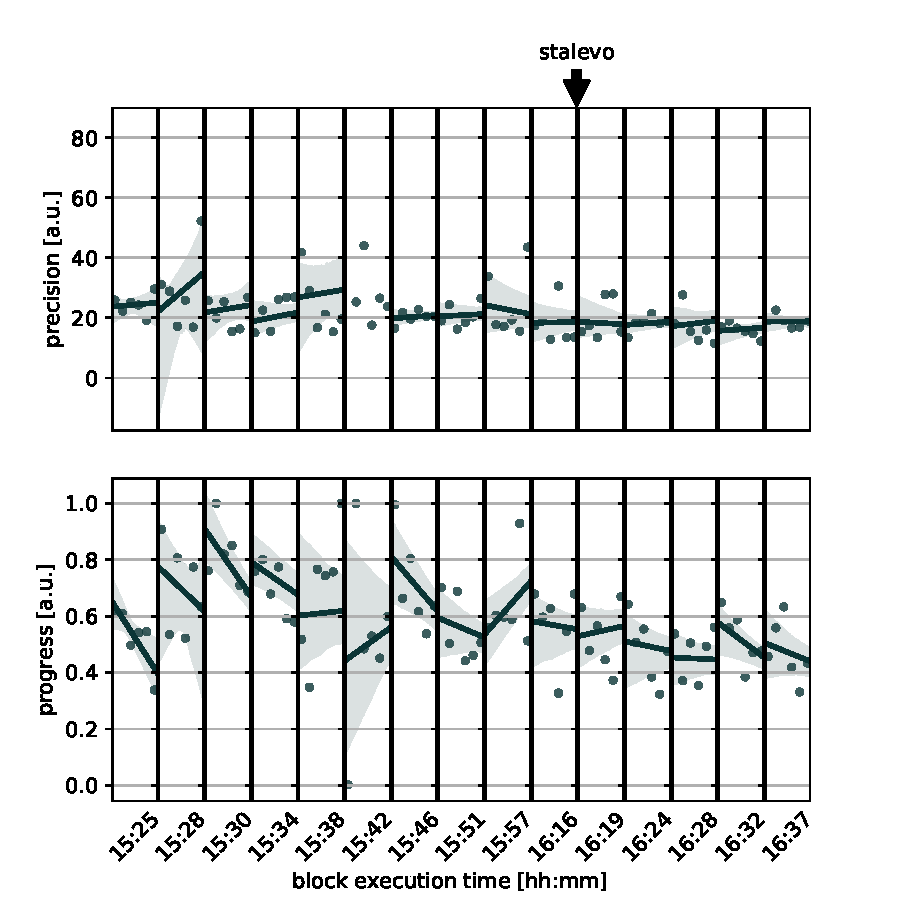
\includegraphics[width=\behwidth\textwidth]{figures/behavioral/d0_scores_copyDraw}&
	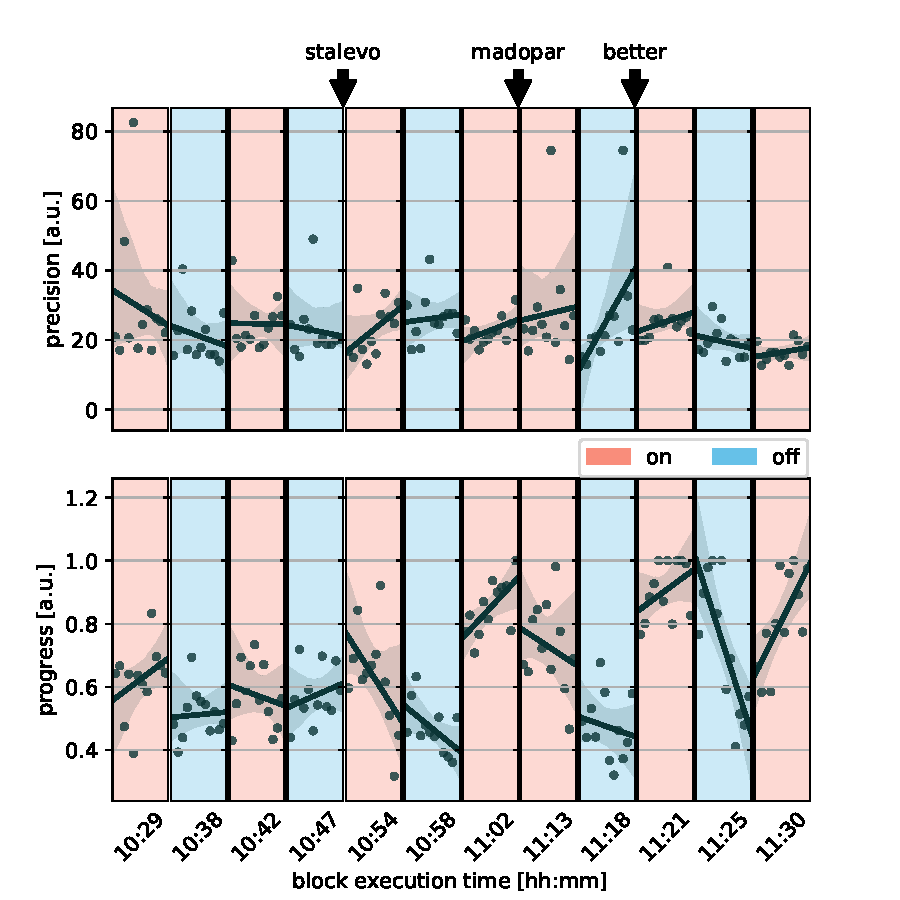
\includegraphics[width=\behwidth\textwidth]{figures/behavioral/d2_scores_copyDraw}&
	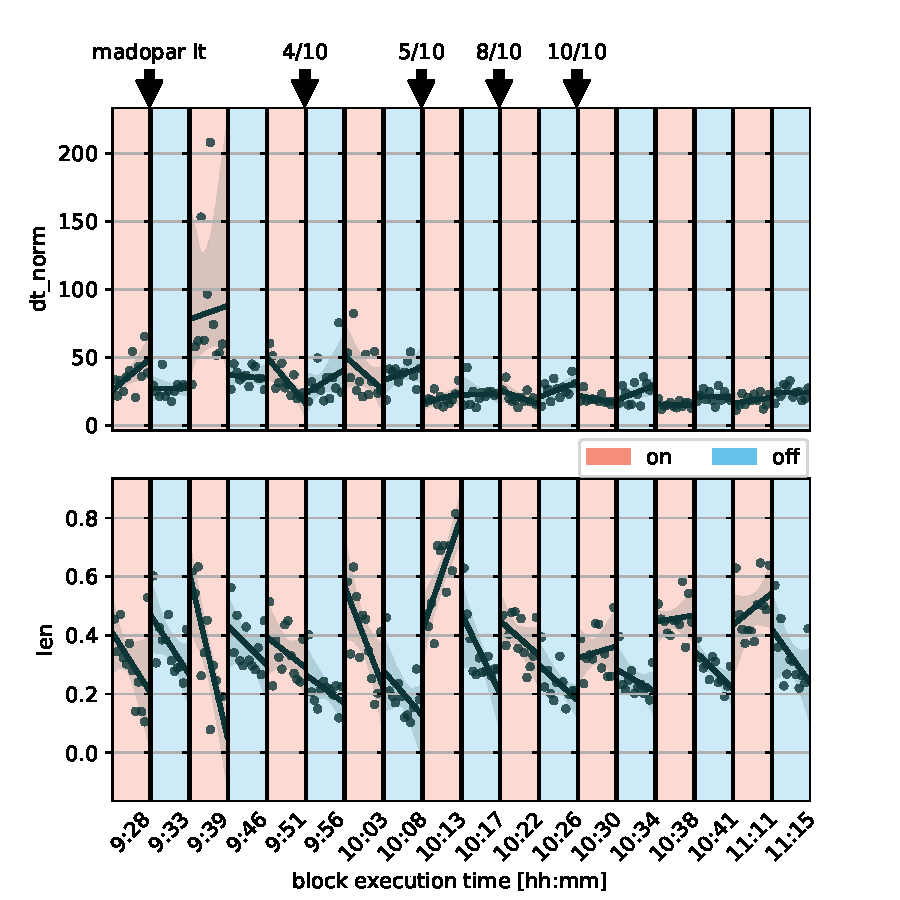
\includegraphics[width=\behwidth\textwidth]{figures/behavioral/d4_scores_copyDraw}
\end{tabular}
\caption{raw performance}
\end{figure}

\begin{figure}
\centering
\begin{tabular}{ccc}
	D0 & D2  & D4 \\
	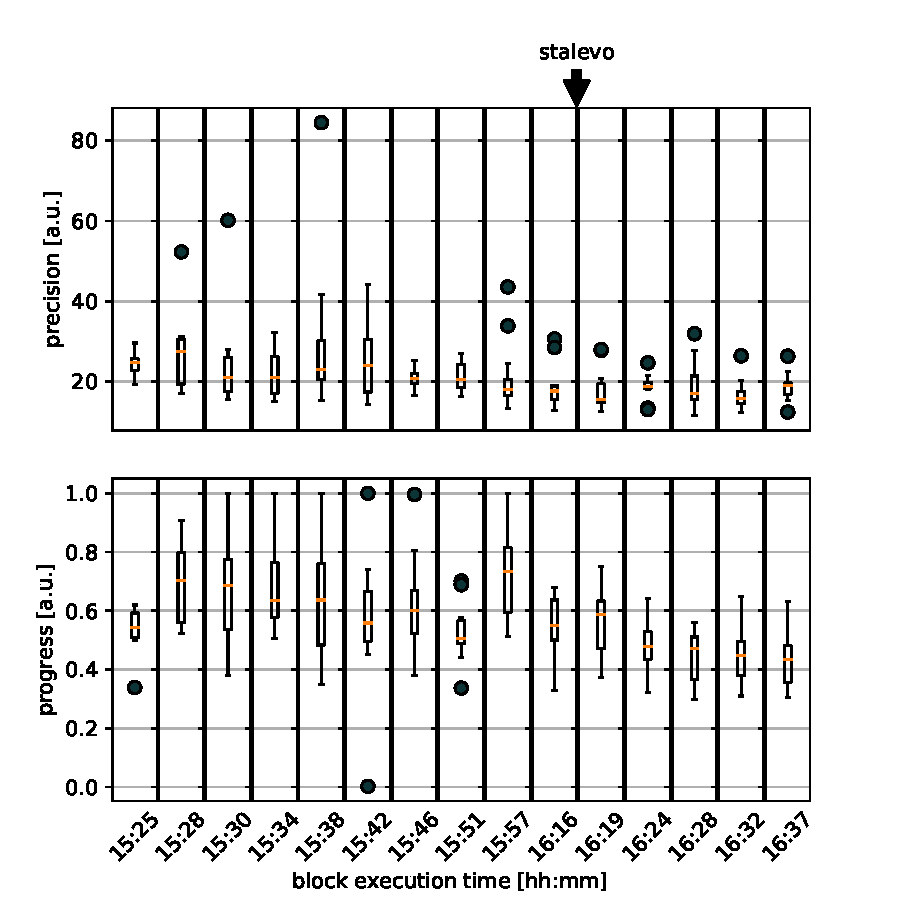
\includegraphics[width=\behwidth\textwidth]{figures/behavioral/d0_stats_scores_copyDraw}&
	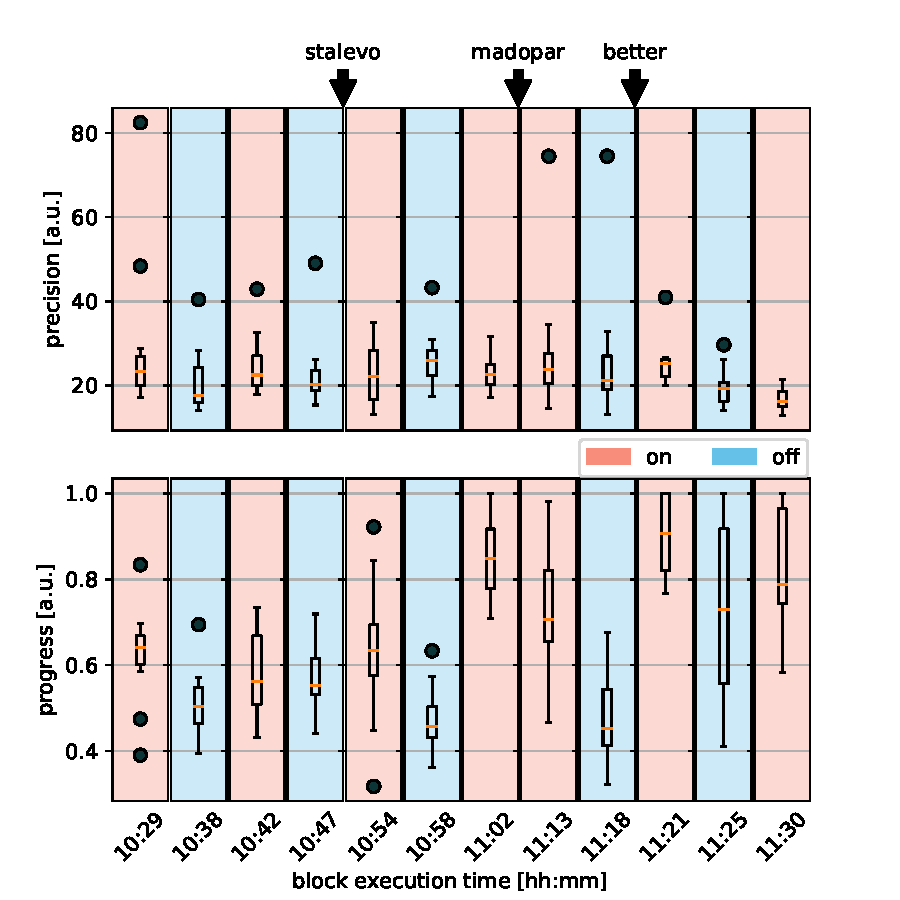
\includegraphics[width=\behwidth\textwidth]{figures/behavioral/d2_stats_scores_copyDraw}&
	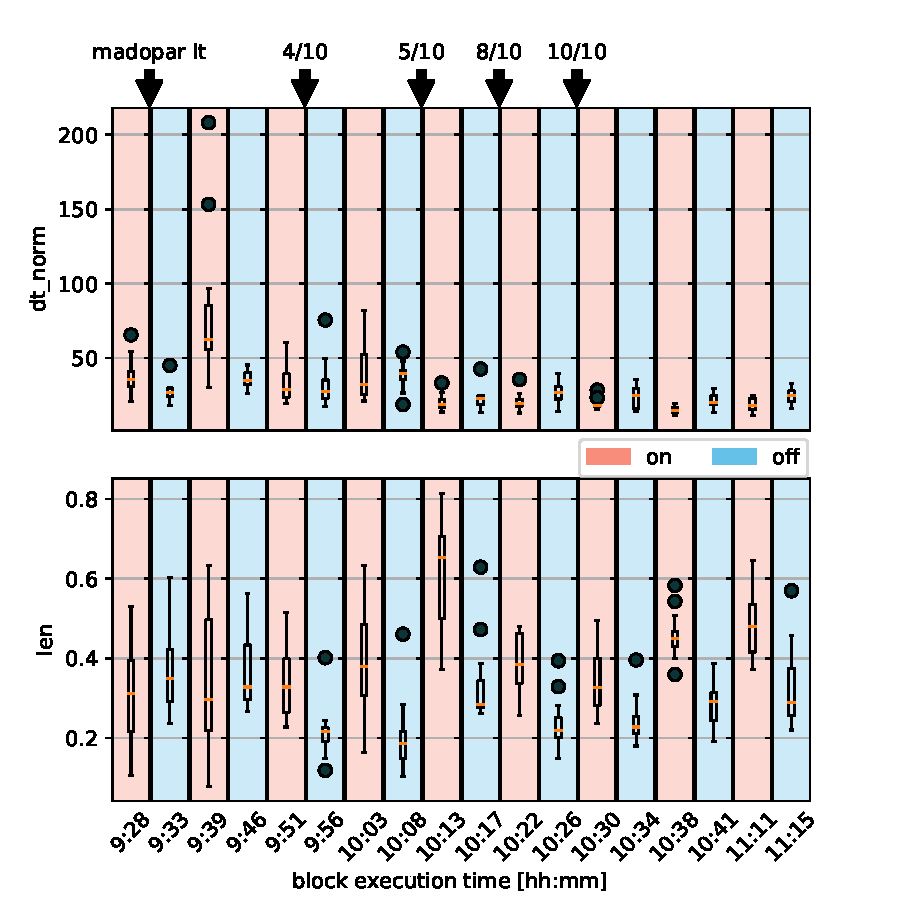
\includegraphics[width=\behwidth\textwidth]{figures//behavioral/d4_stats_scores_copyDraw}
\end{tabular}
\caption{boxplots}
\end{figure}

\newcommand{\perfwidth}{0.99}
\begin{figure}
\centering
\begin{tabular}{c}
	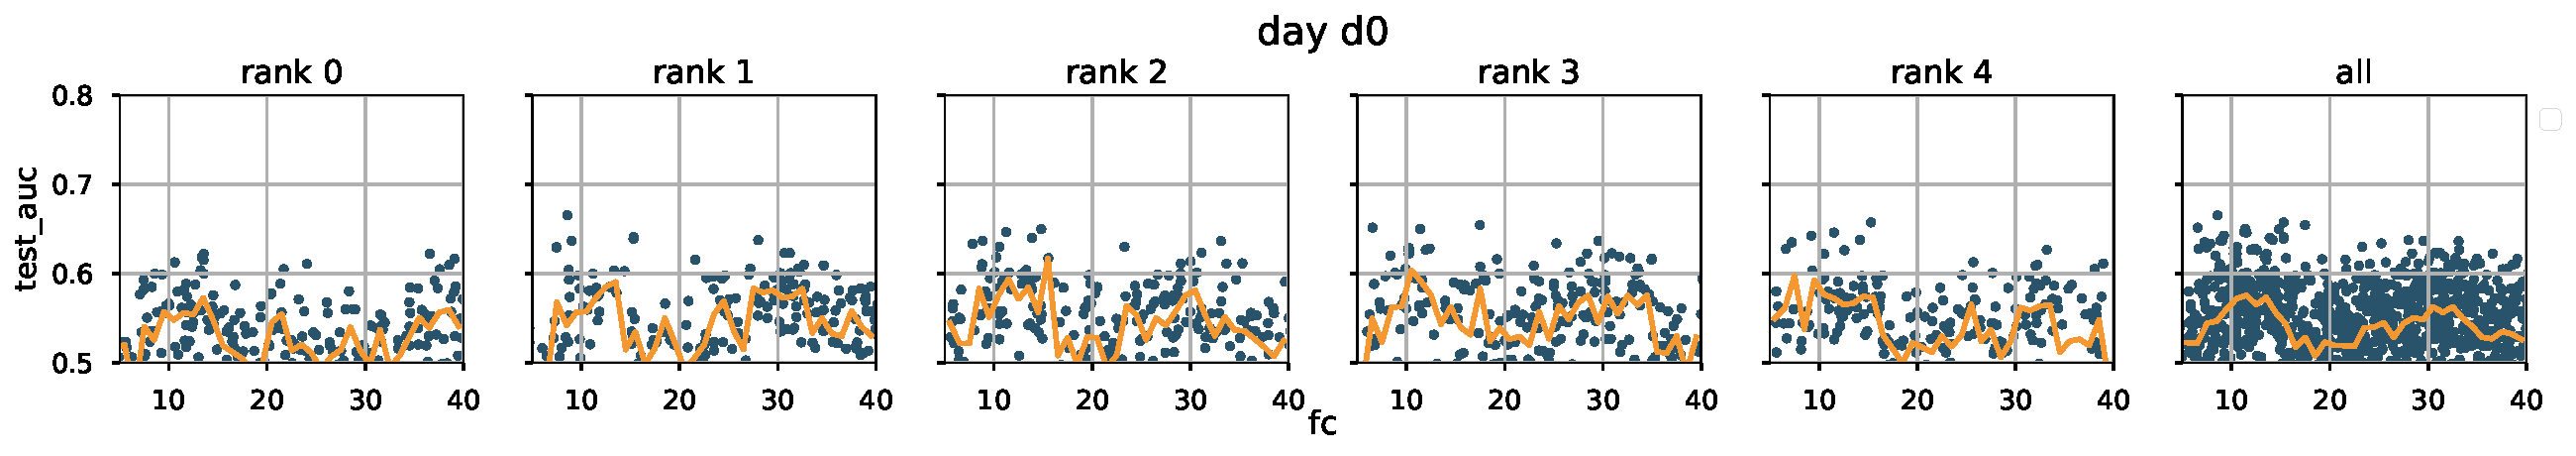
\includegraphics[width=\perfwidth\textwidth]{figures/par_sweep/test_auc_fc_d0_Chrono_Multi}\\
	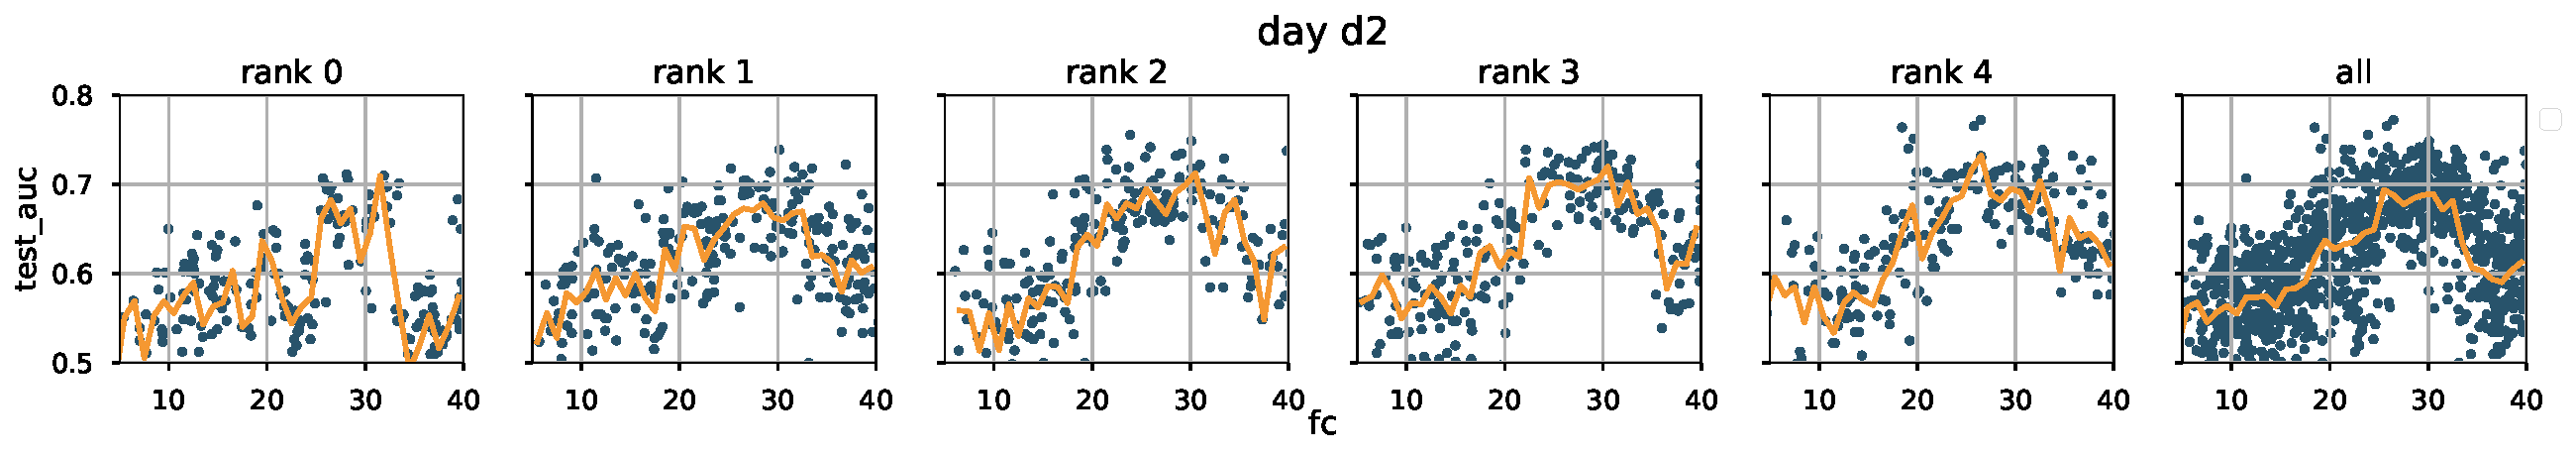
\includegraphics[width=\perfwidth\textwidth]{figures/par_sweep/test_auc_fc_d2_Chrono_Multi}\\
	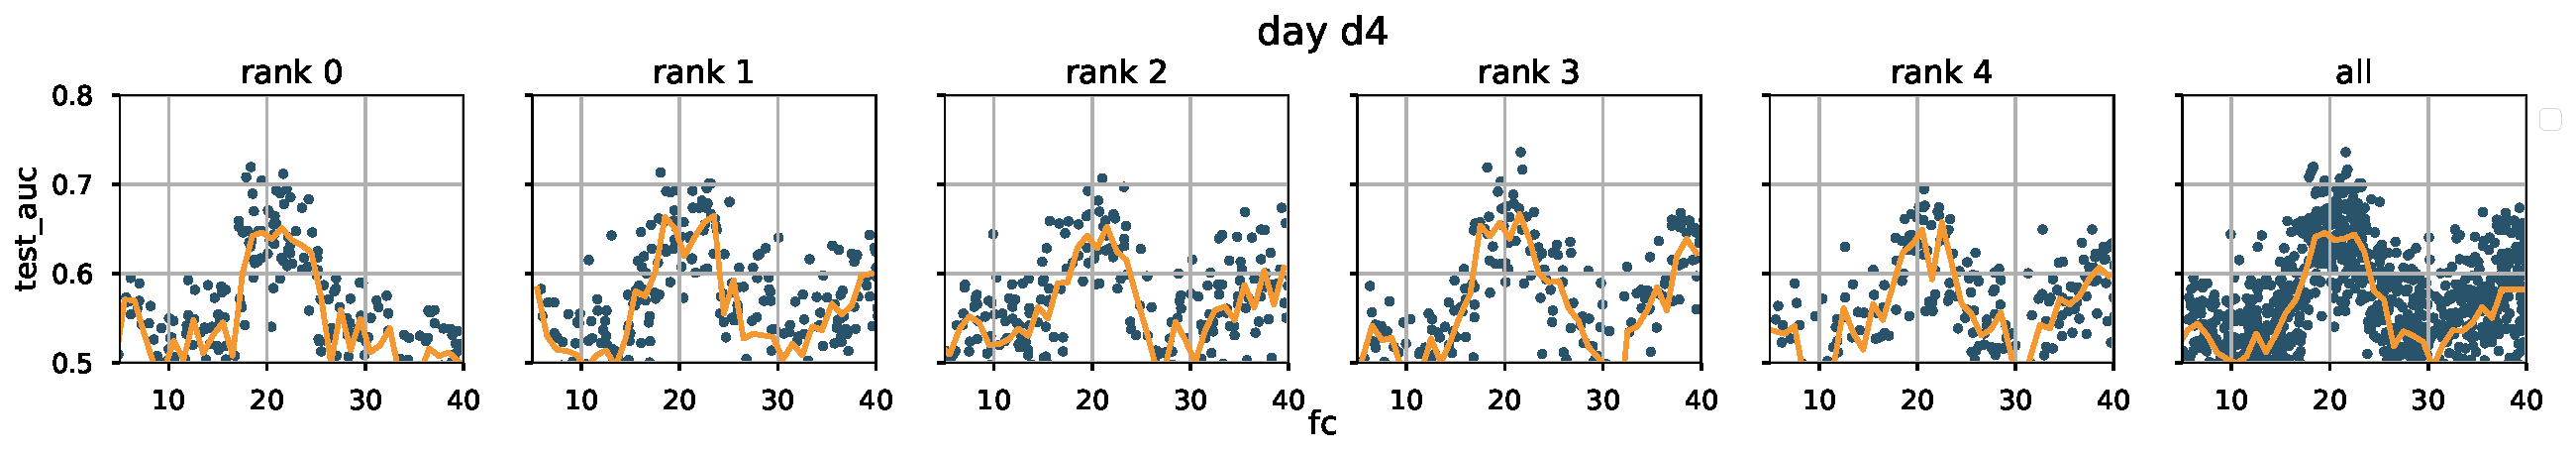
\includegraphics[width=\perfwidth\textwidth]{figures//par_sweep/test_auc_fc_d4_Chrono_Multi}
\end{tabular}
\caption{Chronological xval - AUC -Multi } 
\end{figure}

\begin{figure}
\centering
\begin{tabular}{c}
	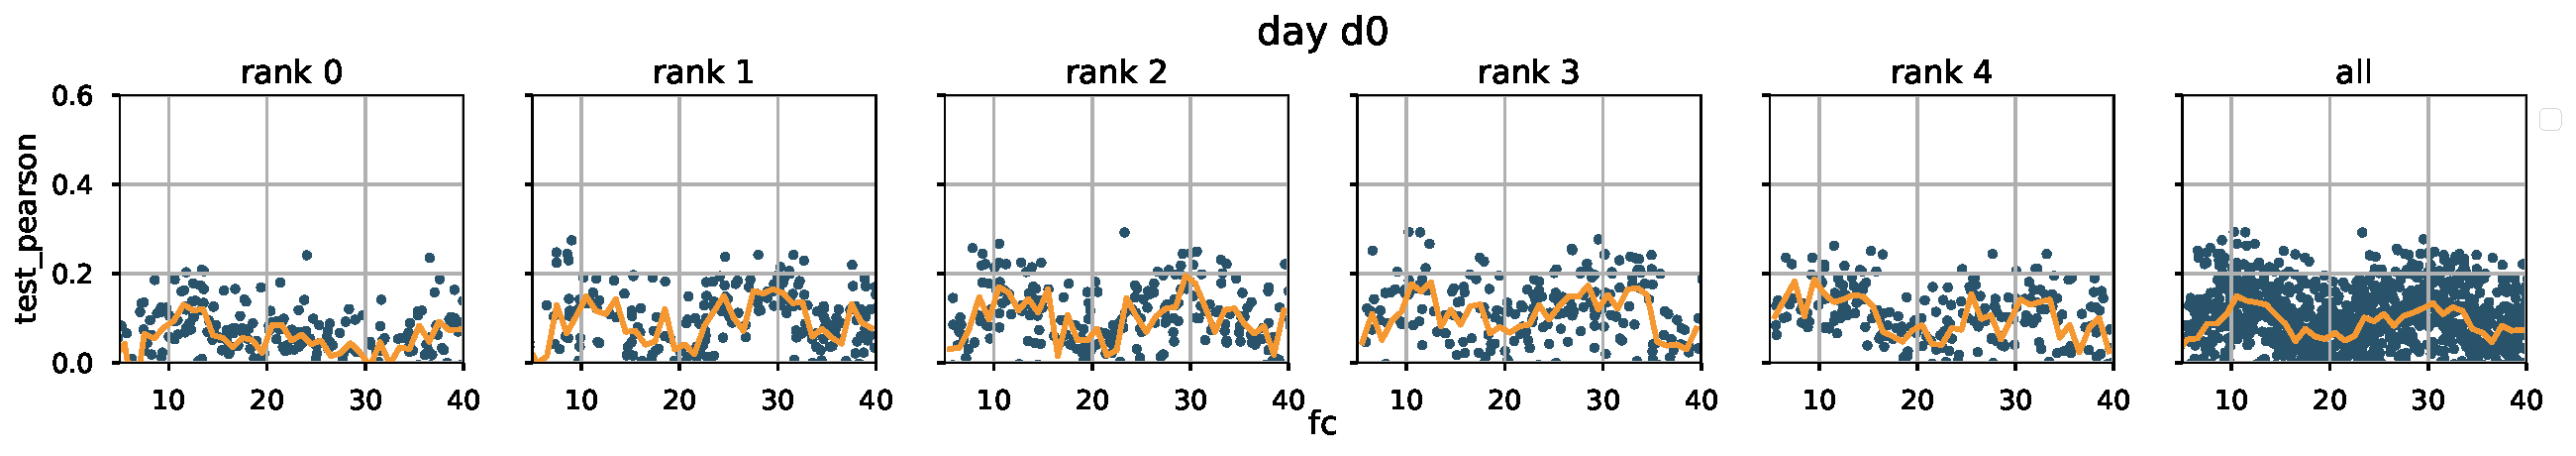
\includegraphics[width=\perfwidth\textwidth]{figures/par_sweep/test_pearson_fc_d0_Chrono_Multi}\\
	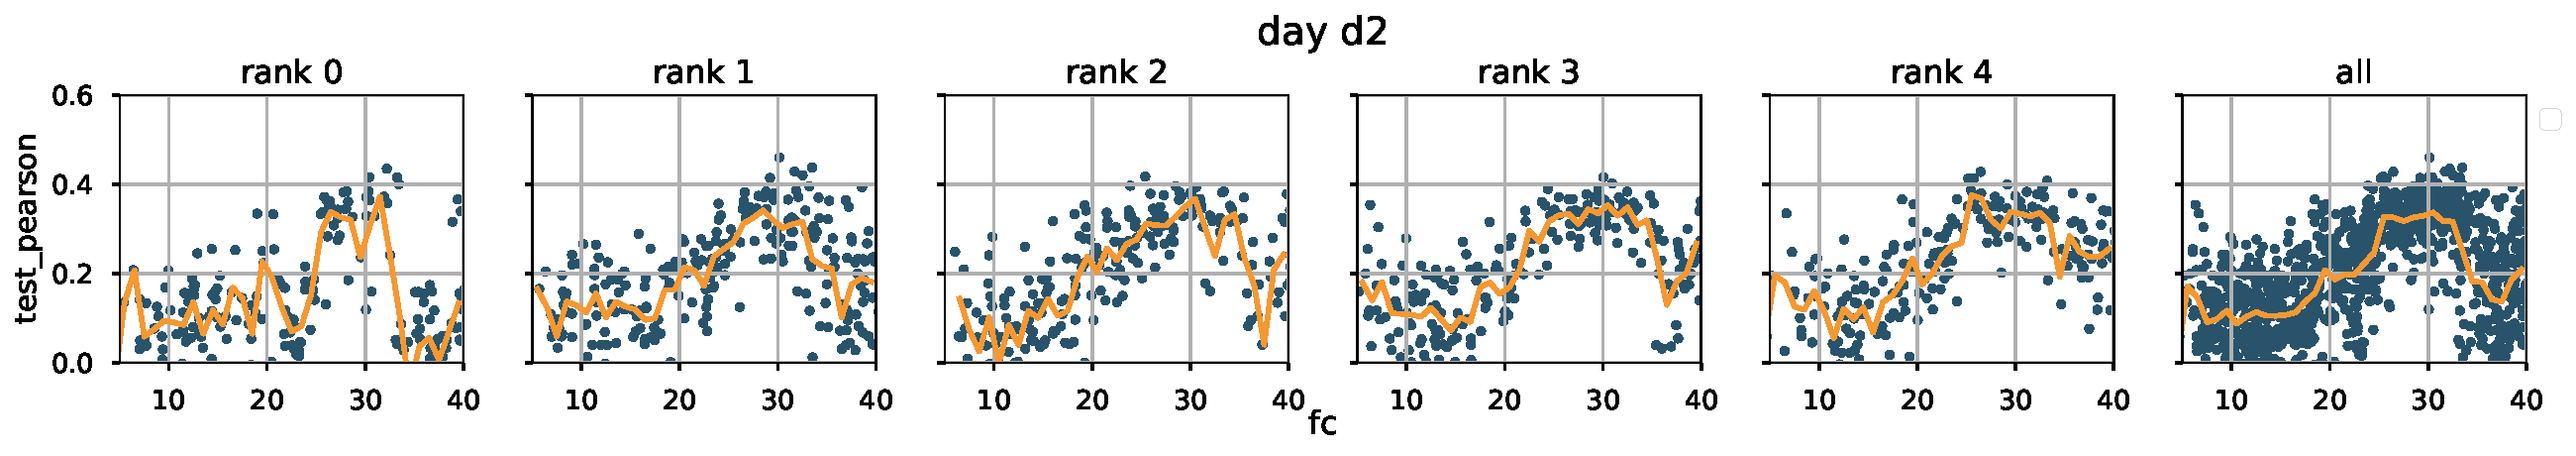
\includegraphics[width=\perfwidth\textwidth]{figures/par_sweep/test_pearson_fc_d2_Chrono_Multi}\\
	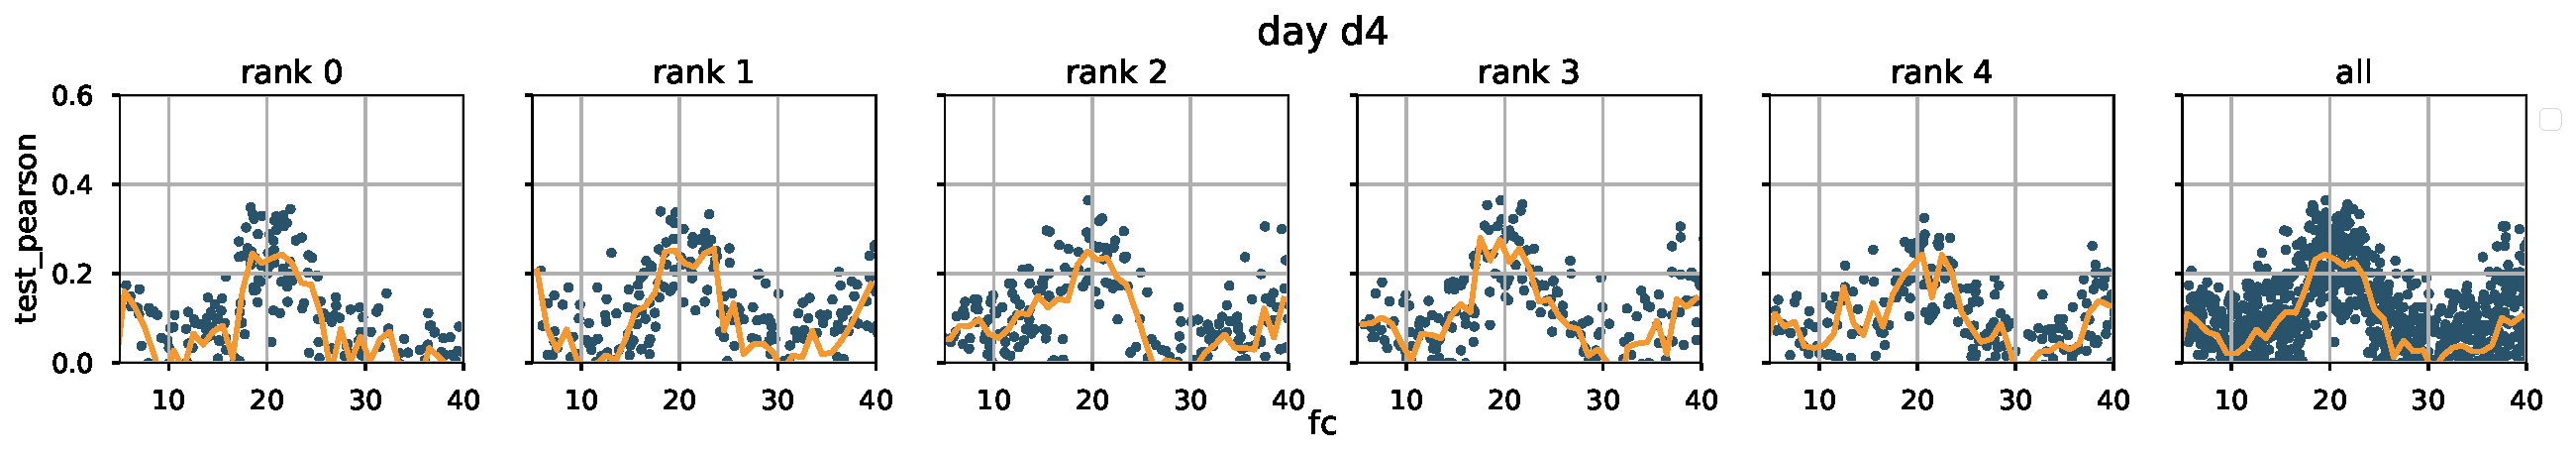
\includegraphics[width=\perfwidth\textwidth]{figures//par_sweep/test_pearson_fc_d4_Chrono_Multi}
\end{tabular}
\caption{Chronological xval - Pearson -Multi} 
\end{figure}

\begin{figure}
\centering
\begin{tabular}{c}
	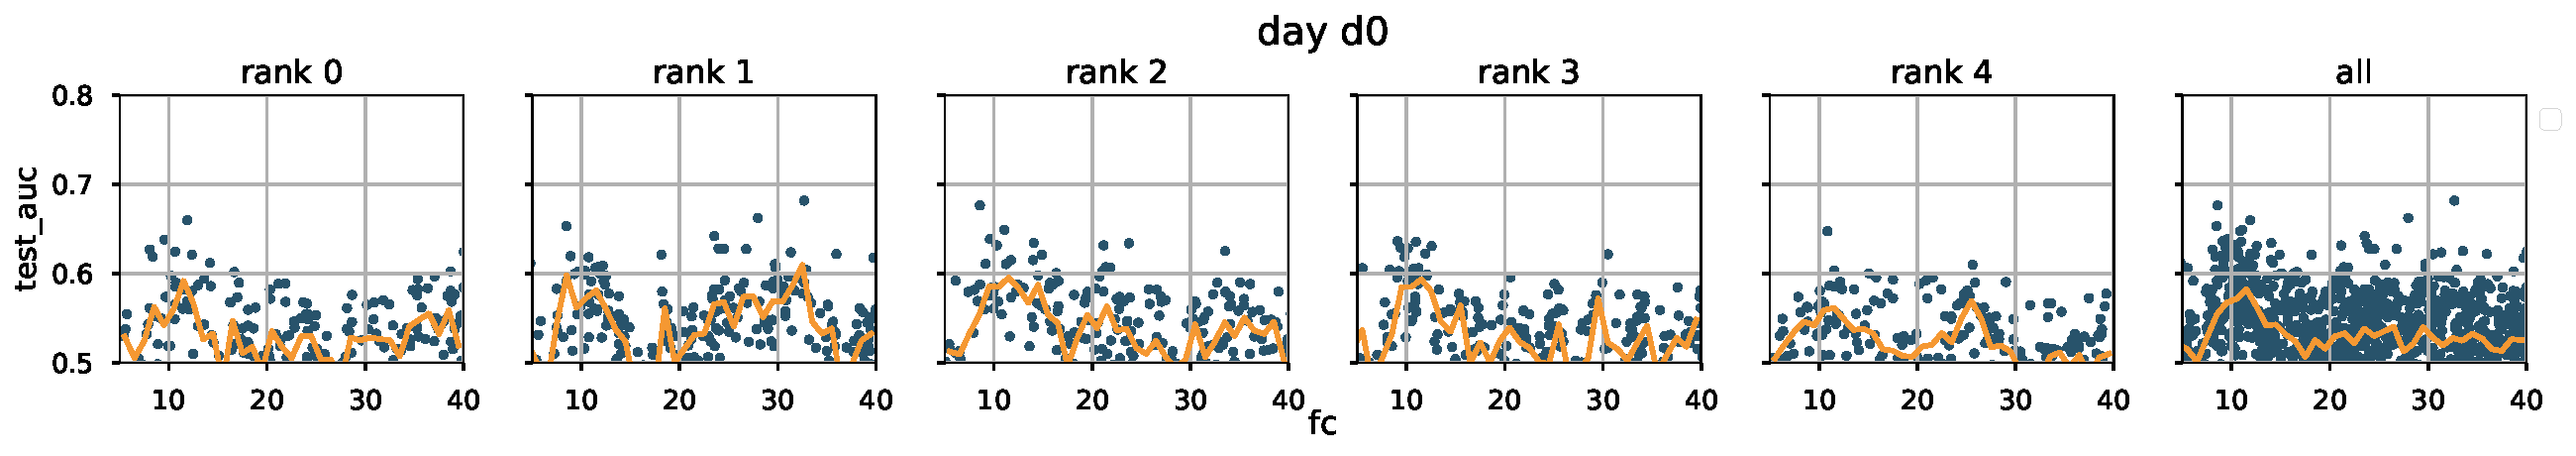
\includegraphics[width=\perfwidth\textwidth]{figures/par_sweep/test_auc_fc_d0_Chrono_Single}\\
	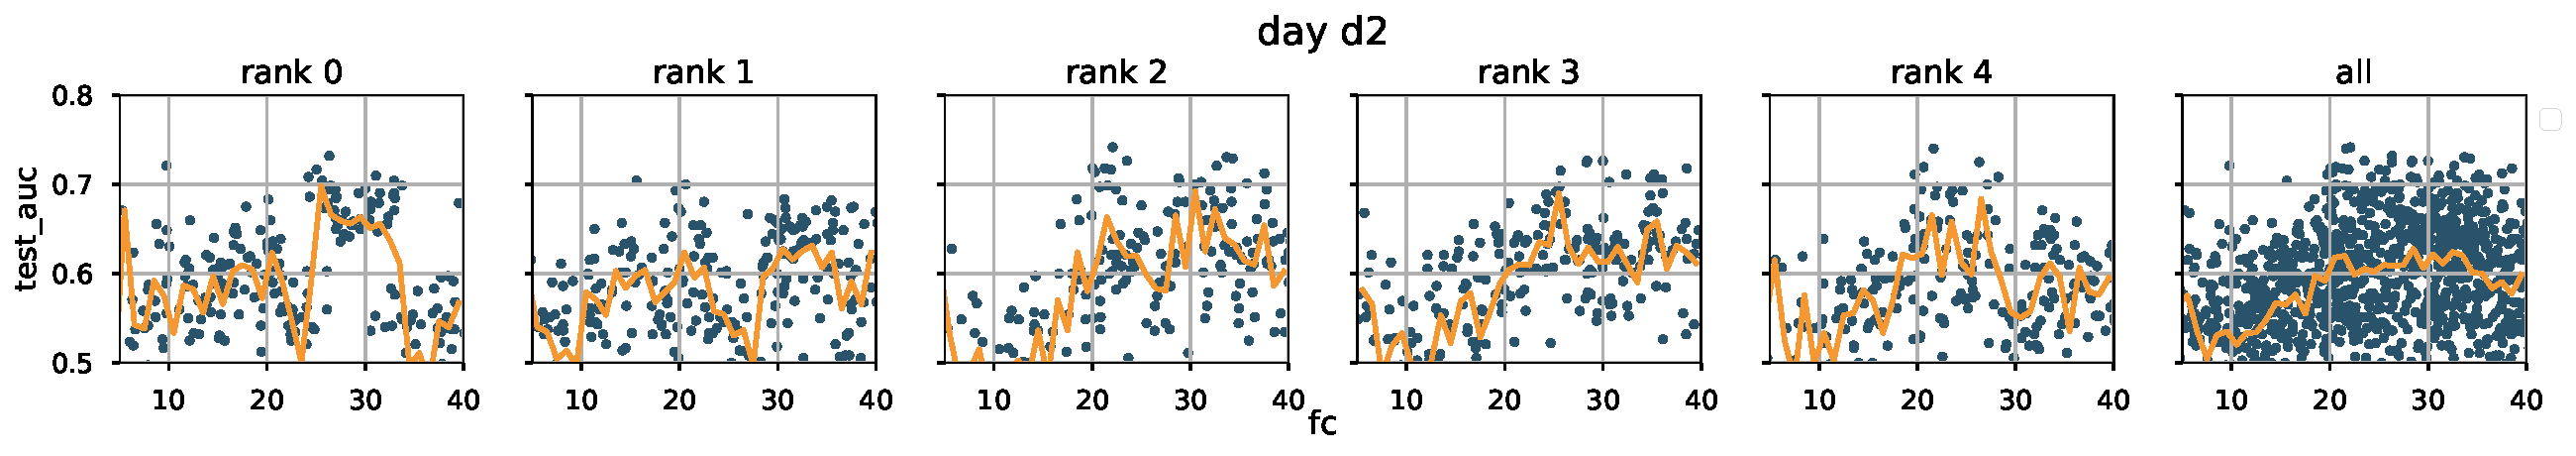
\includegraphics[width=\perfwidth\textwidth]{figures/par_sweep/test_auc_fc_d2_Chrono_Single}\\
	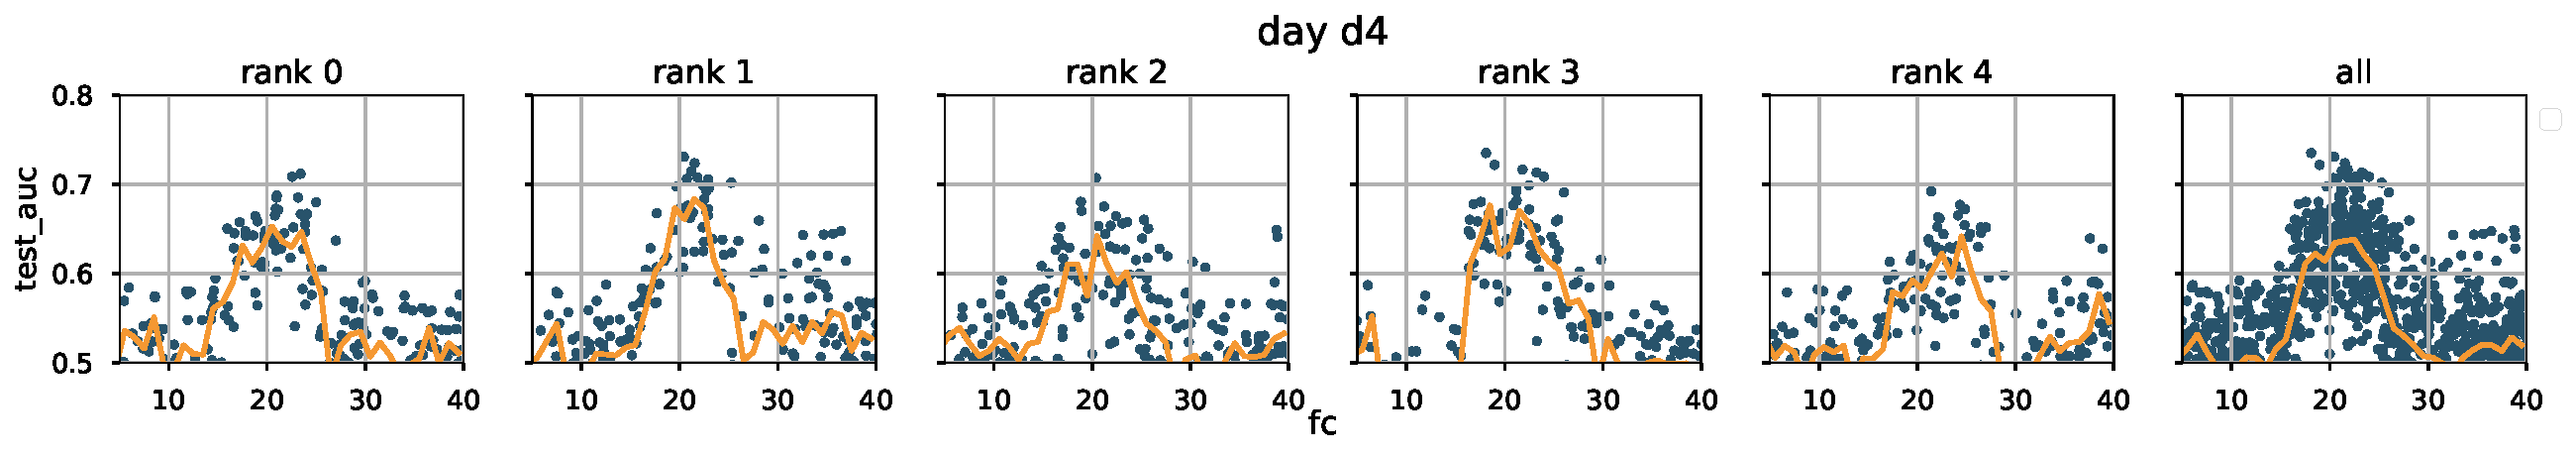
\includegraphics[width=\perfwidth\textwidth]{figures//par_sweep/test_auc_fc_d4_Chrono_Single}
\end{tabular}
\caption{Chronological xval - AUC - Single} 
\end{figure}

\begin{figure}
\centering
\begin{tabular}{c}
	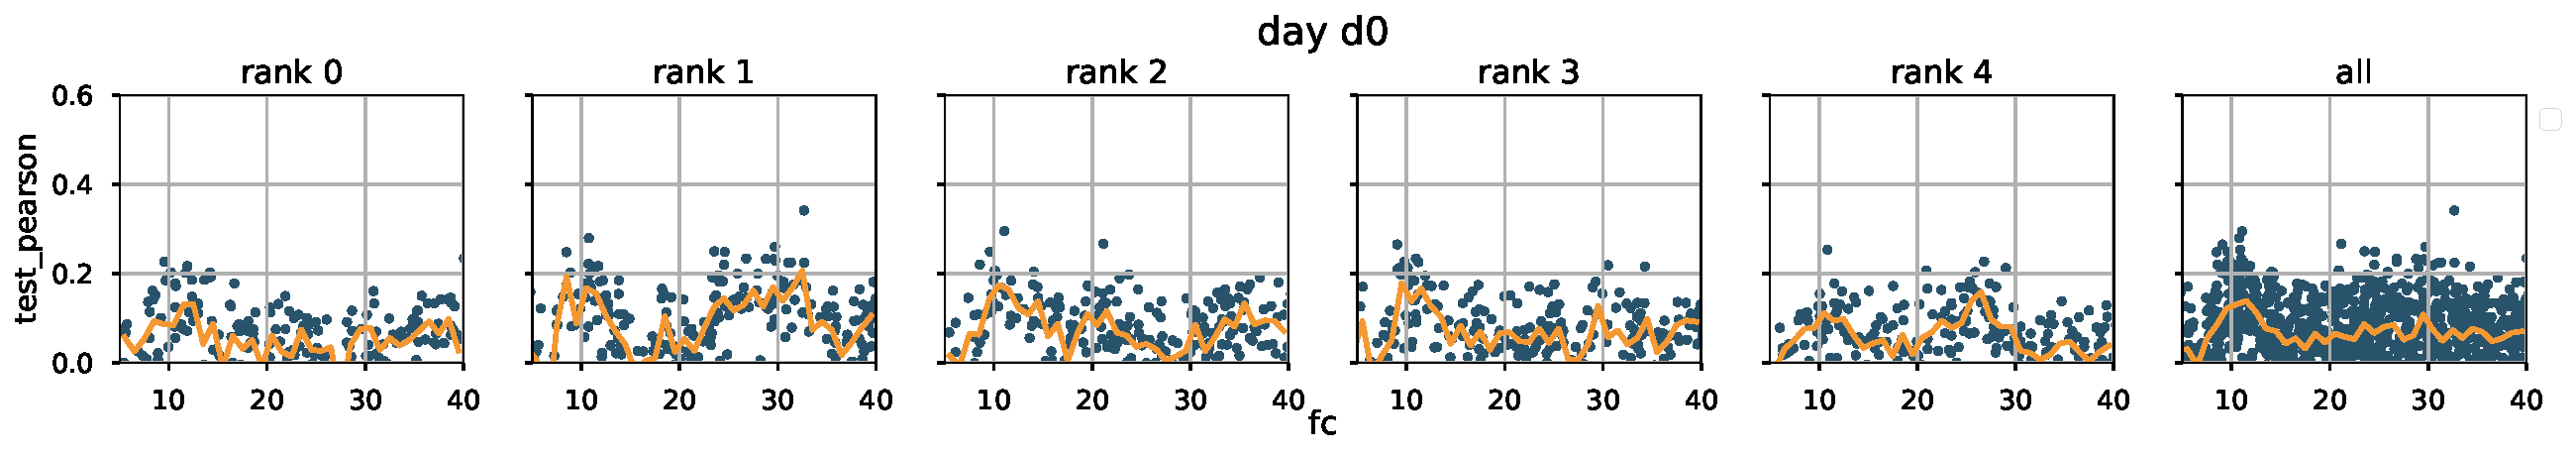
\includegraphics[width=\perfwidth\textwidth]{figures/par_sweep/test_pearson_fc_d0_Chrono_Single}\\
	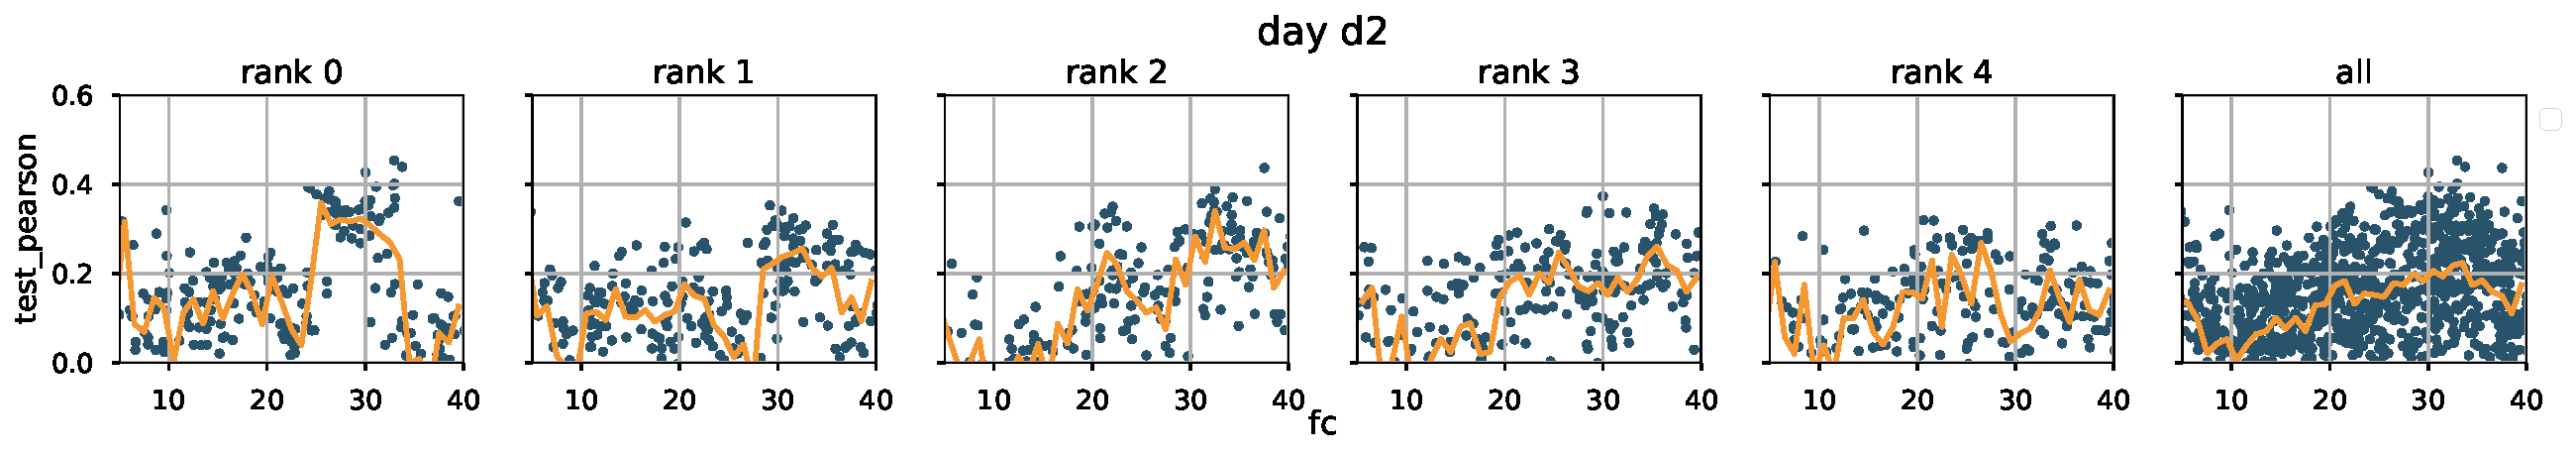
\includegraphics[width=\perfwidth\textwidth]{figures/par_sweep/test_pearson_fc_d2_Chrono_Single}\\
	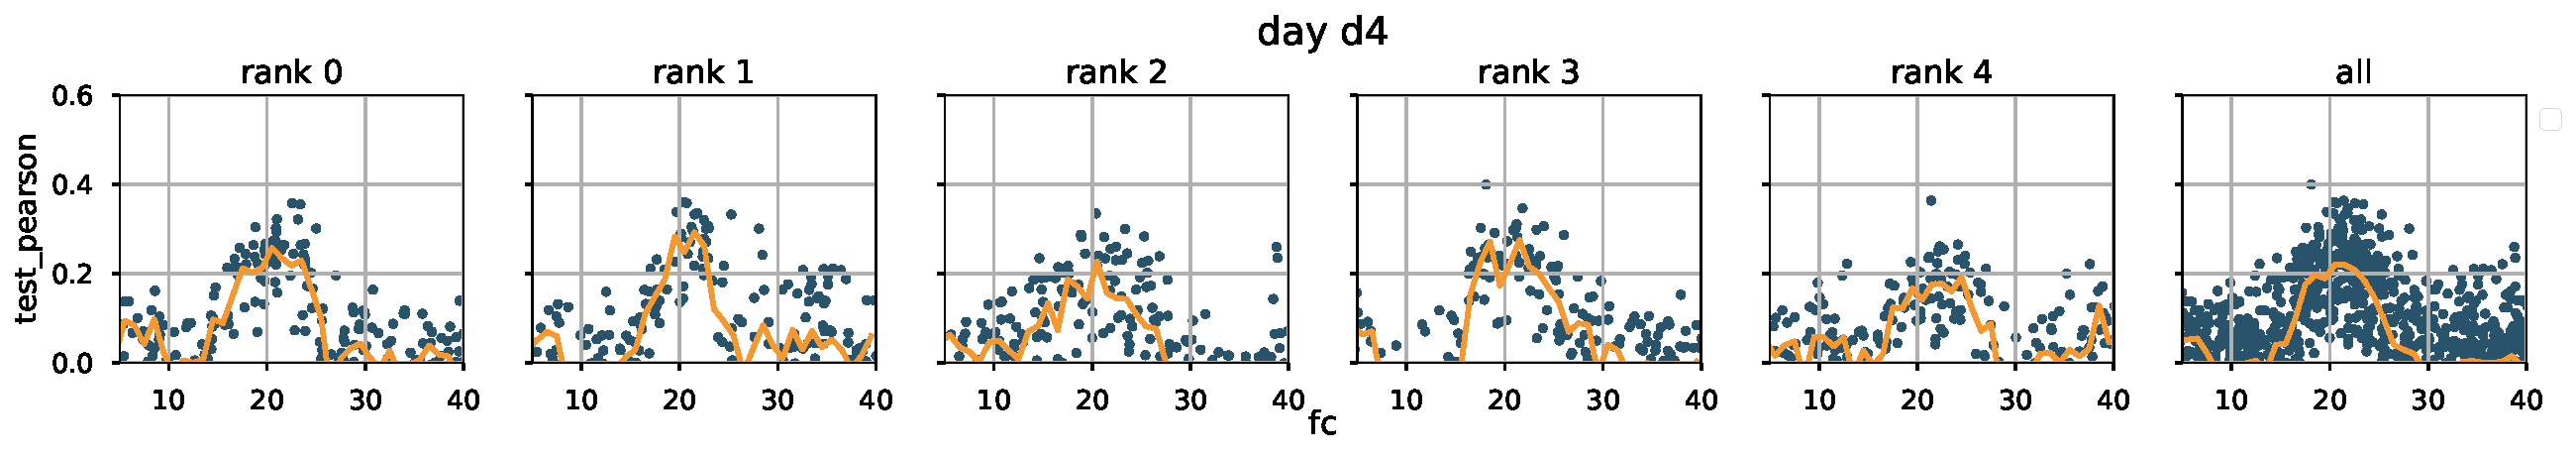
\includegraphics[width=\perfwidth\textwidth]{figures//par_sweep/test_pearson_fc_d4_Chrono_Single}
\end{tabular}
\caption{Chronological xval - Pearson - Single} 
\end{figure}

%--------------------------------- %
\begin{figure}
\centering
\begin{tabular}{c}
	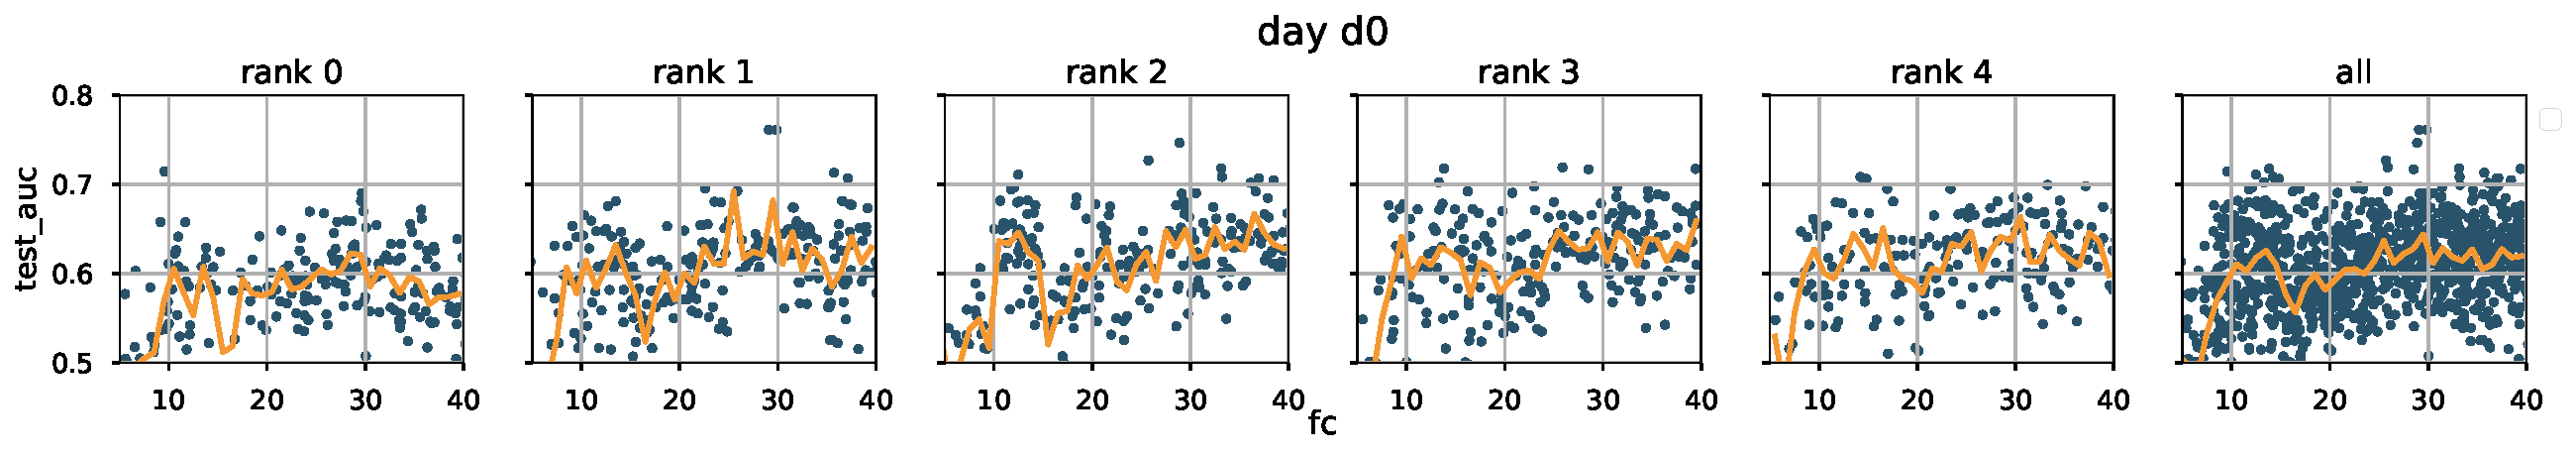
\includegraphics[width=\perfwidth\textwidth]{figures/par_sweep/test_auc_fc_d0_Shuffle_Multi}\\
	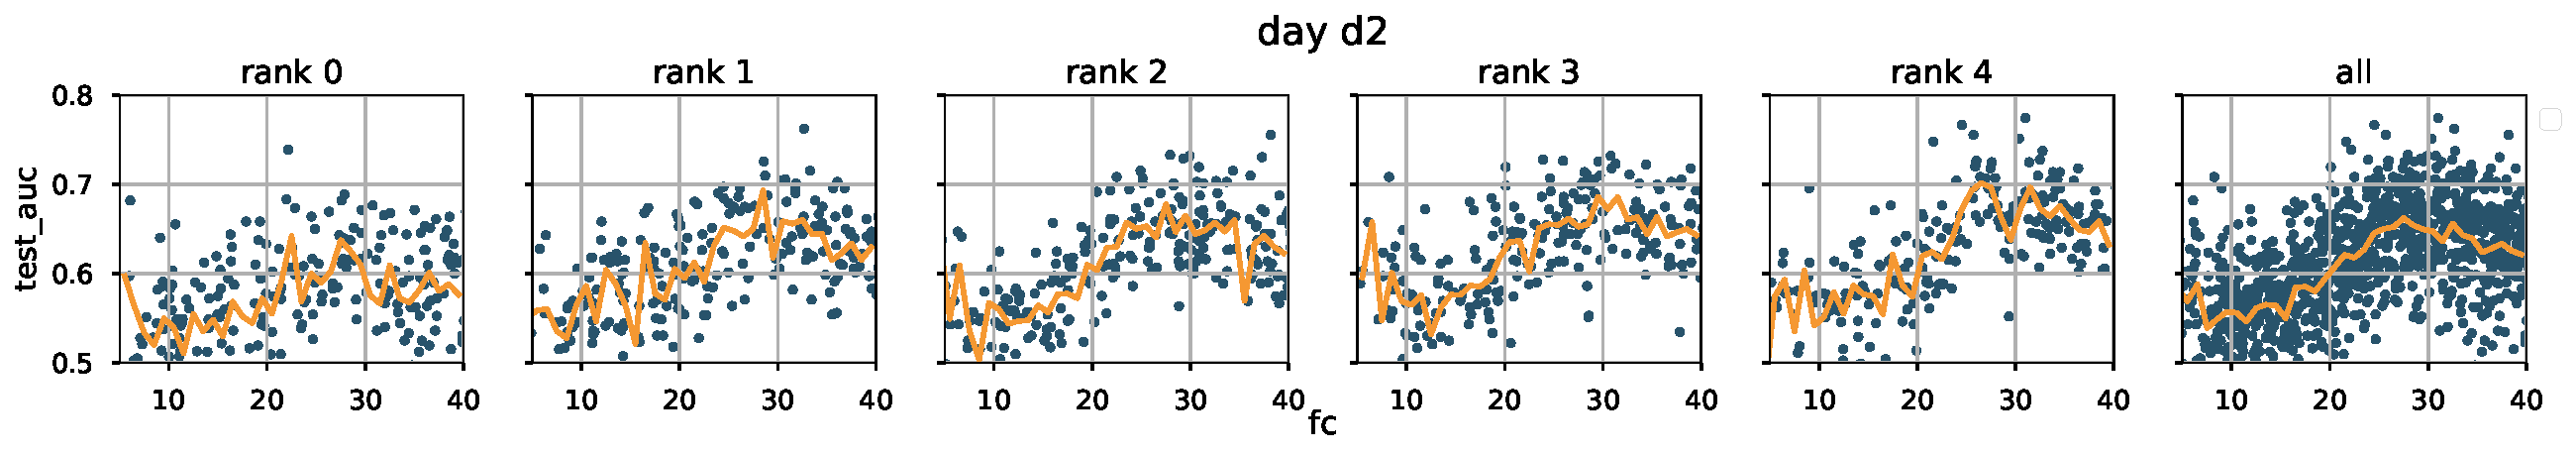
\includegraphics[width=\perfwidth\textwidth]{figures/par_sweep/test_auc_fc_d2_Shuffle_Multi}\\
	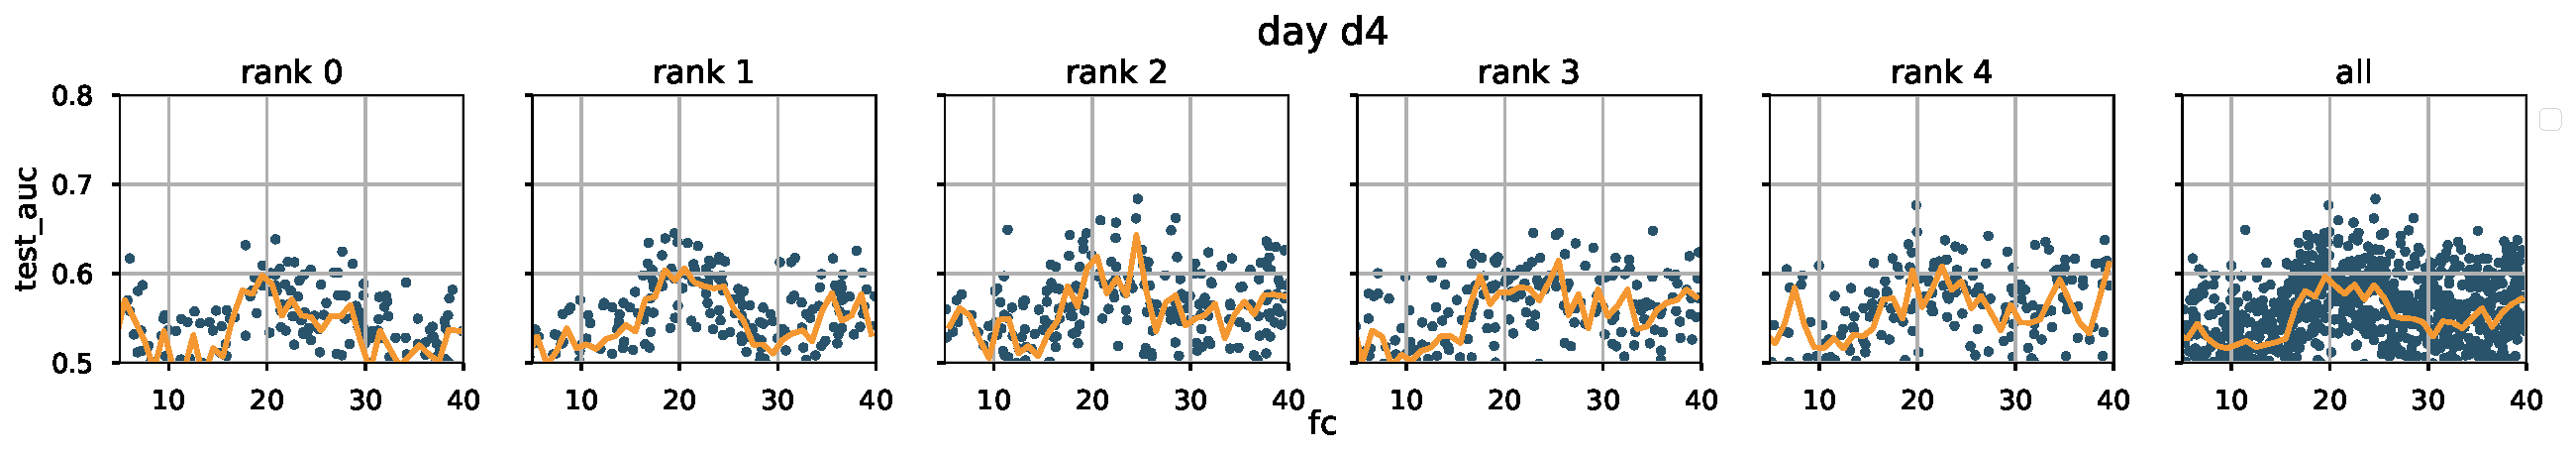
\includegraphics[width=\perfwidth\textwidth]{figures//par_sweep/test_auc_fc_d4_Shuffle_Multi}
\end{tabular}
\caption{Shuffle xval - AUC -Multi } 
\end{figure}

\begin{figure}
\centering
\begin{tabular}{c}
	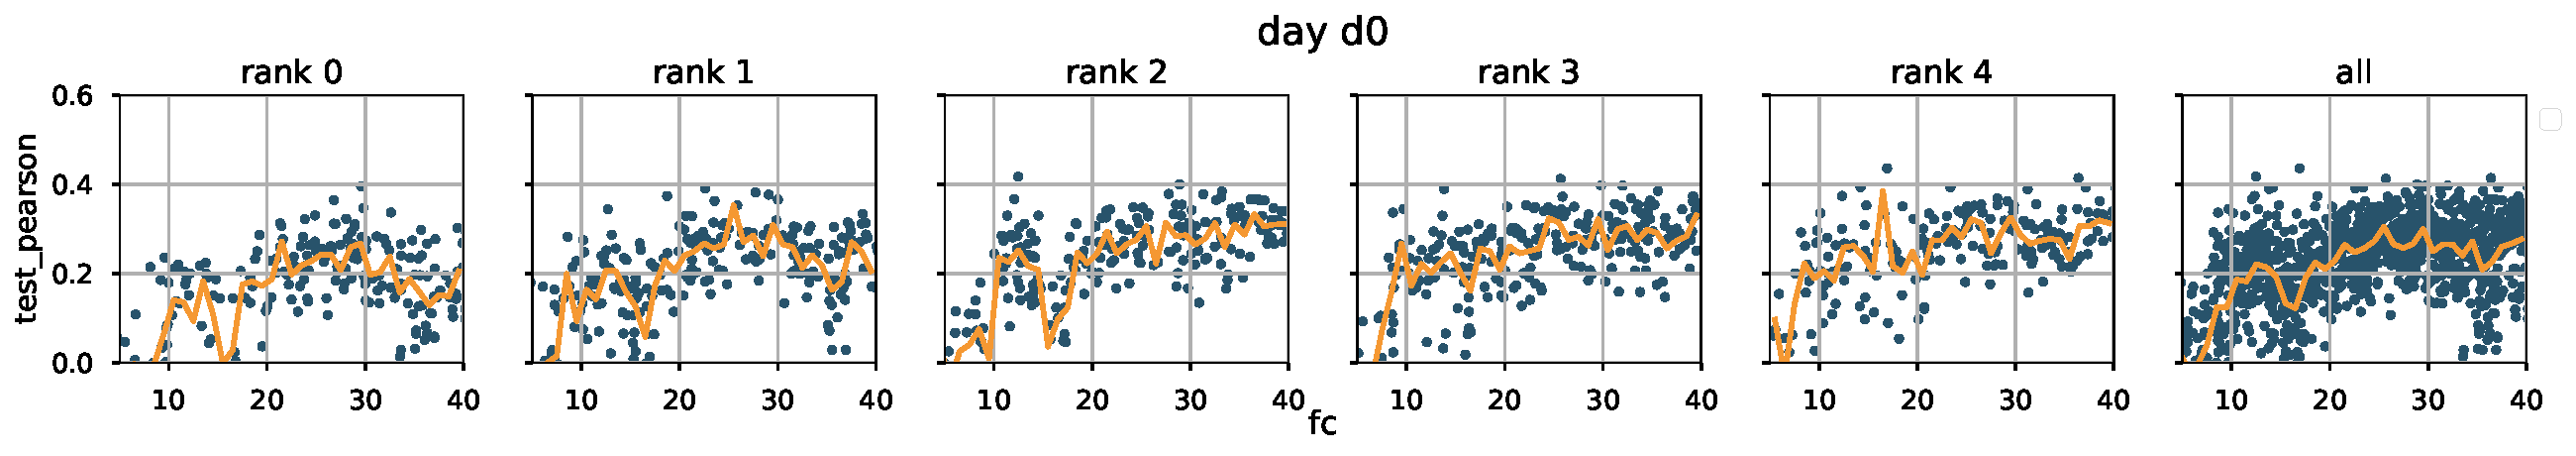
\includegraphics[width=\perfwidth\textwidth]{figures/par_sweep/test_pearson_fc_d0_Shuffle_Multi}\\
	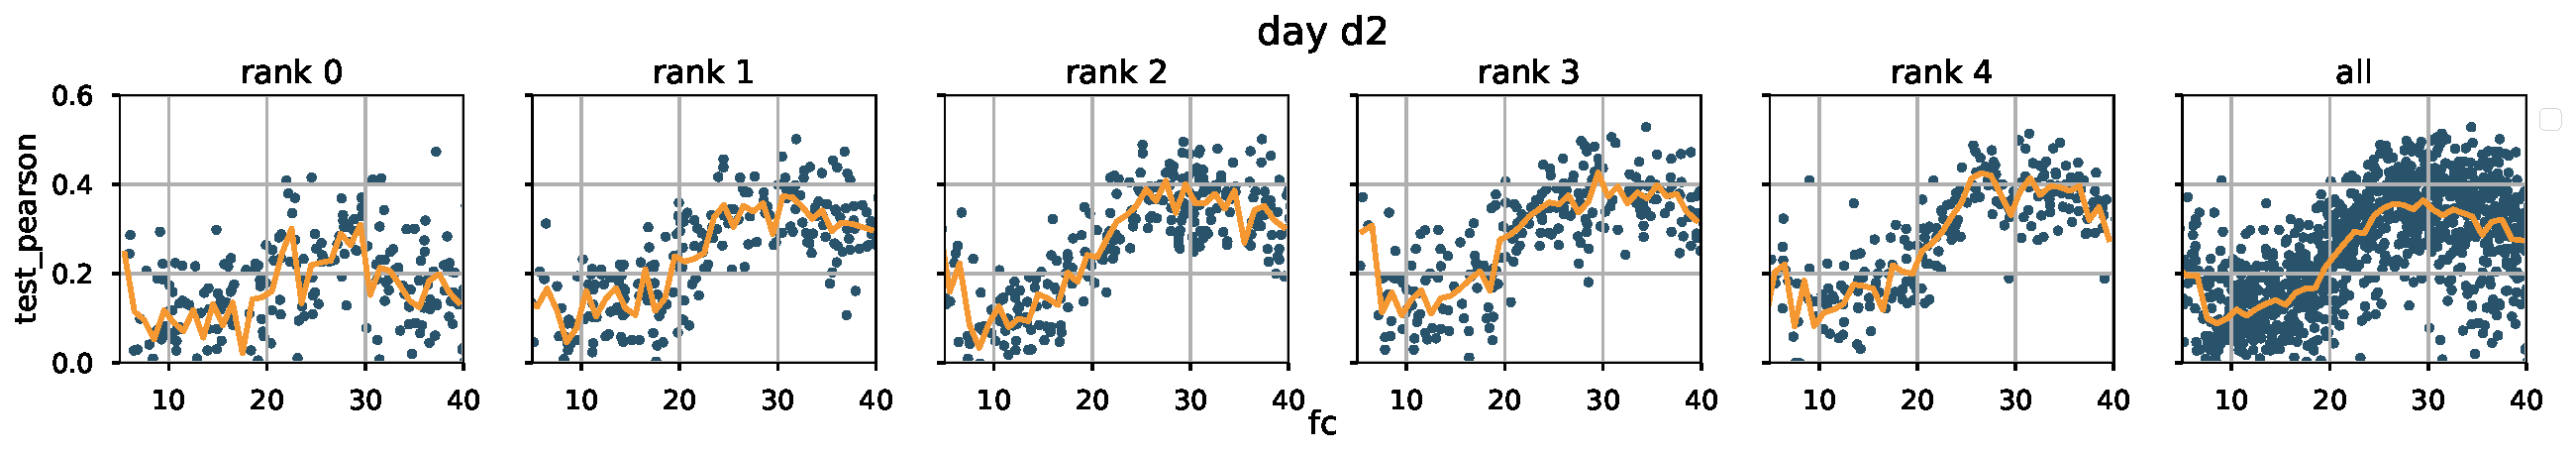
\includegraphics[width=\perfwidth\textwidth]{figures/par_sweep/test_pearson_fc_d2_Shuffle_Multi}\\
	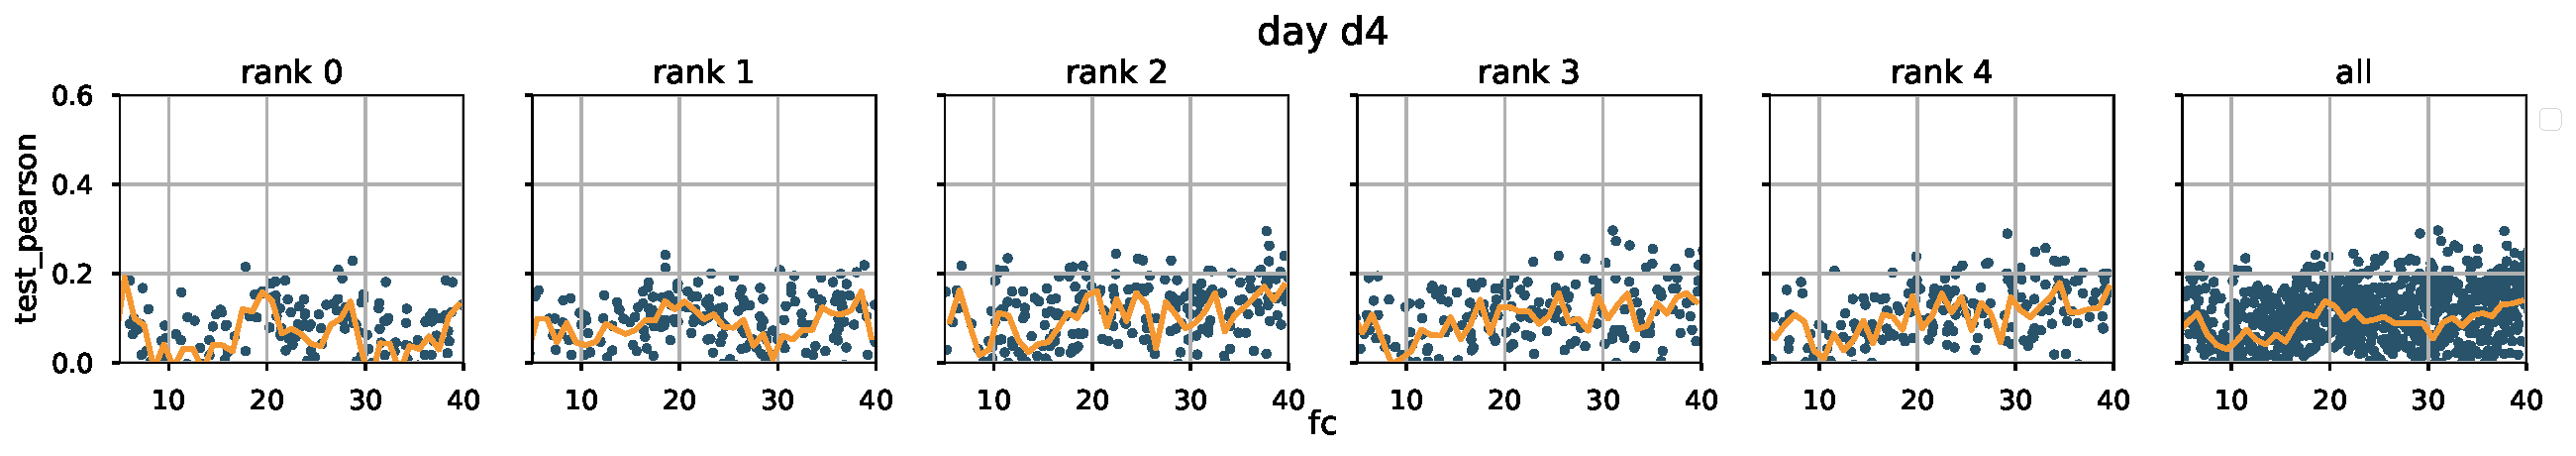
\includegraphics[width=\perfwidth\textwidth]{figures//par_sweep/test_pearson_fc_d4_Shuffle_Multi}
\end{tabular}
\caption{Shuffle xval - Pearson -Multi} 
\end{figure}

\begin{figure}
\centering
\begin{tabular}{c}
	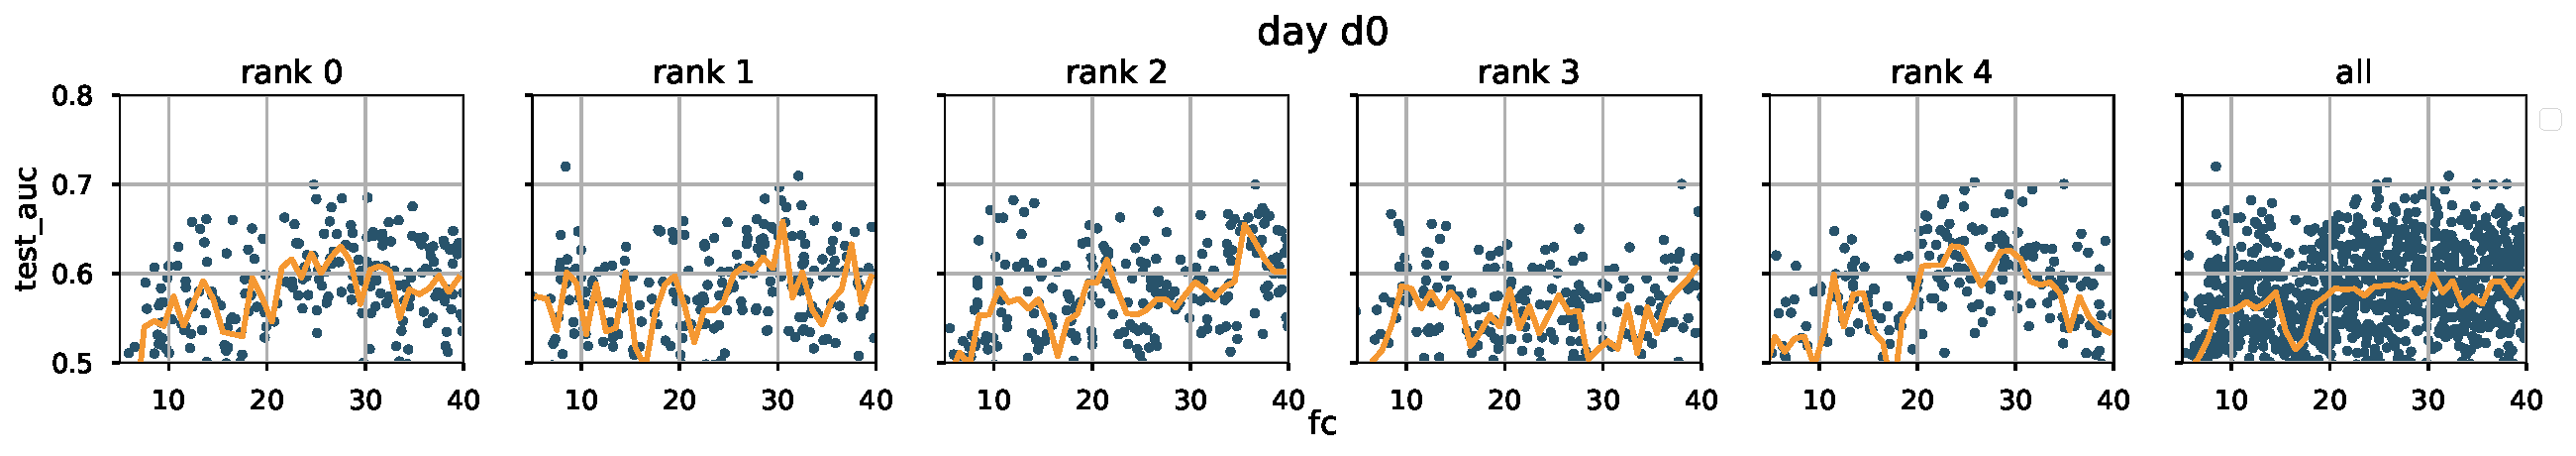
\includegraphics[width=\perfwidth\textwidth]{figures/par_sweep/test_auc_fc_d0_Shuffle_Single}\\
	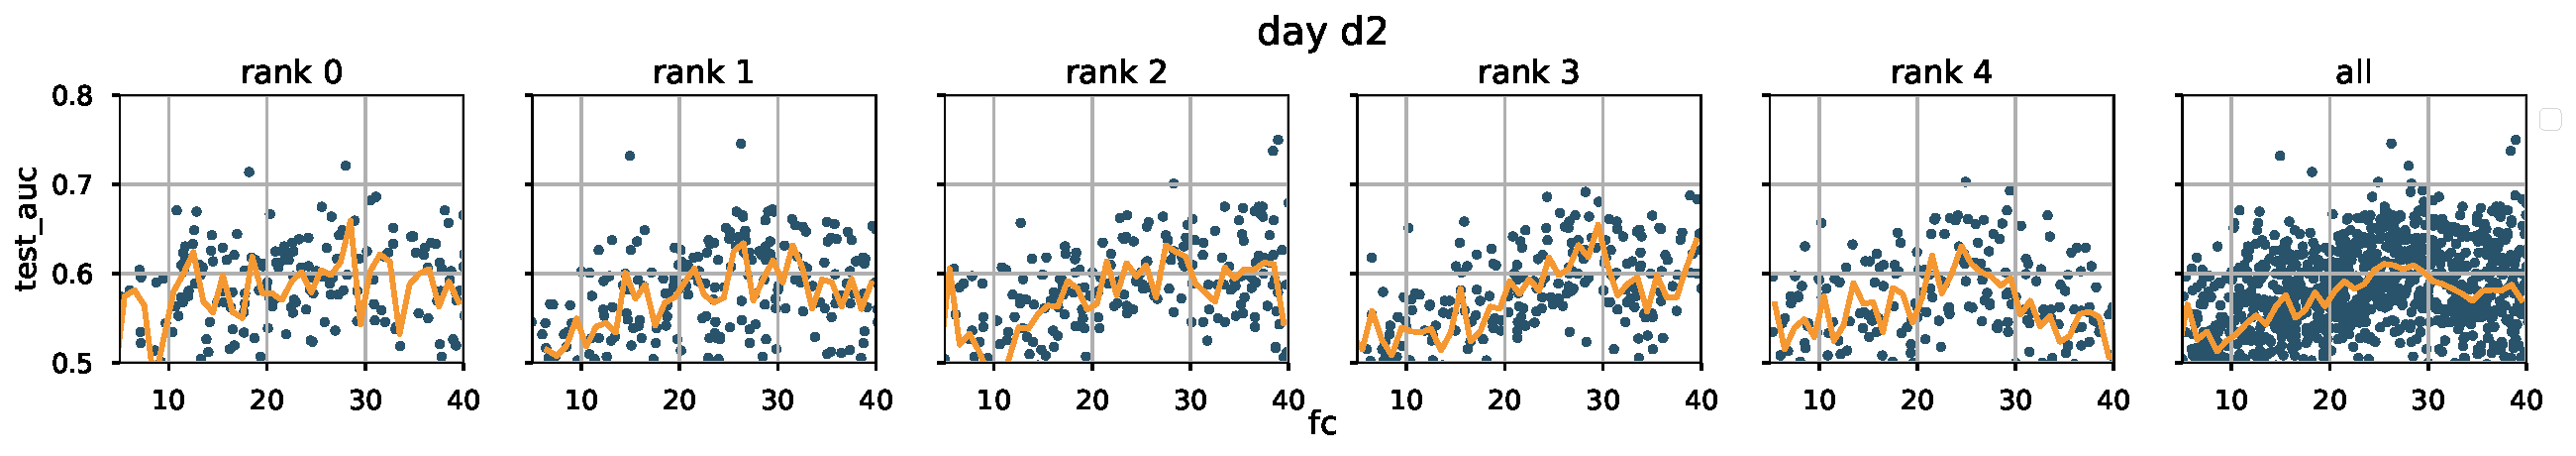
\includegraphics[width=\perfwidth\textwidth]{figures/par_sweep/test_auc_fc_d2_Shuffle_Single}\\
	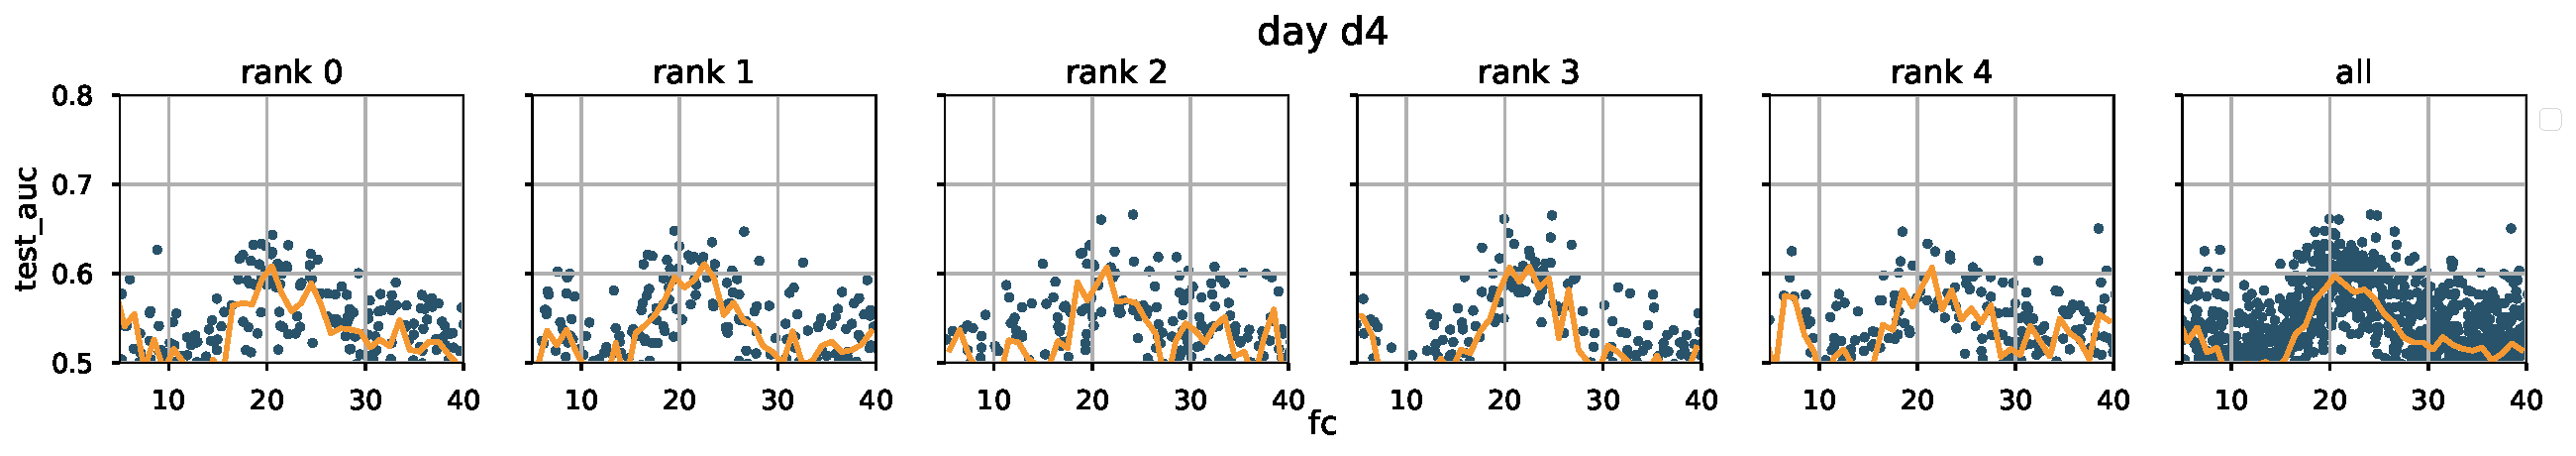
\includegraphics[width=\perfwidth\textwidth]{figures//par_sweep/test_auc_fc_d4_Shuffle_Single}
\end{tabular}
\caption{Shuffle xval - AUC - Single} 
\end{figure}

\begin{figure}
\centering
\begin{tabular}{c}
	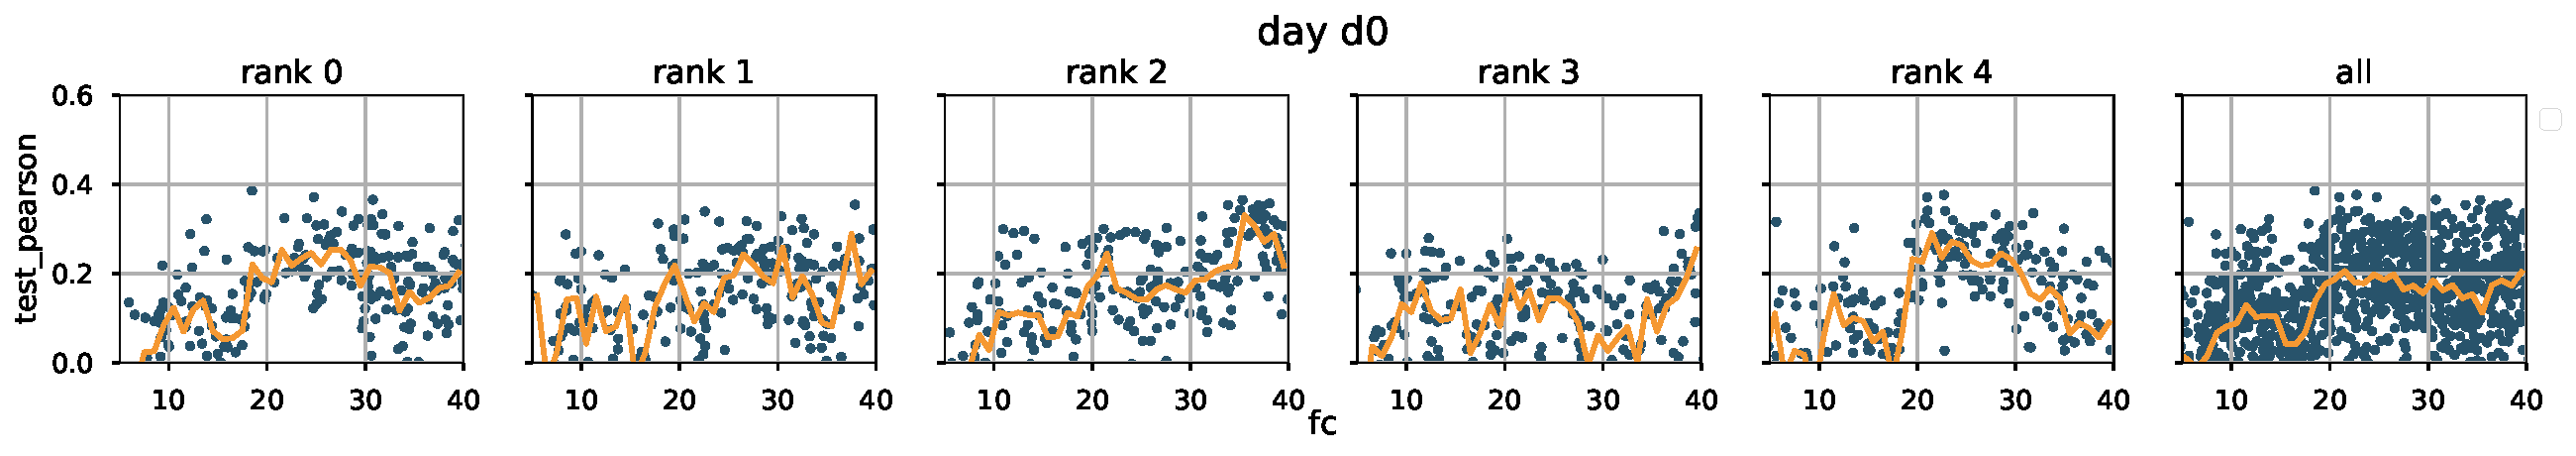
\includegraphics[width=\perfwidth\textwidth]{figures/par_sweep/test_pearson_fc_d0_Shuffle_Single}\\
	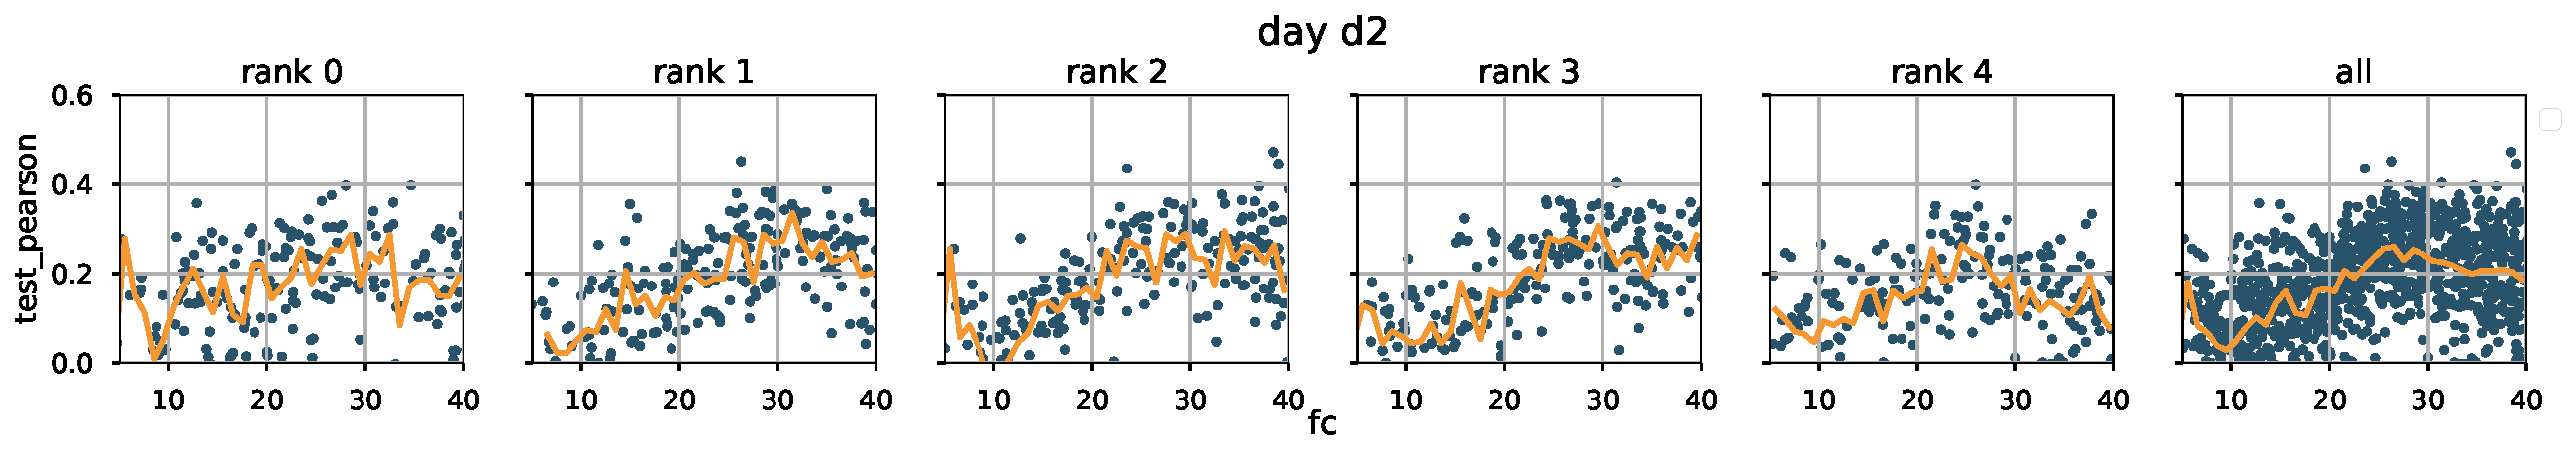
\includegraphics[width=\perfwidth\textwidth]{figures/par_sweep/test_pearson_fc_d2_Shuffle_Single}\\
	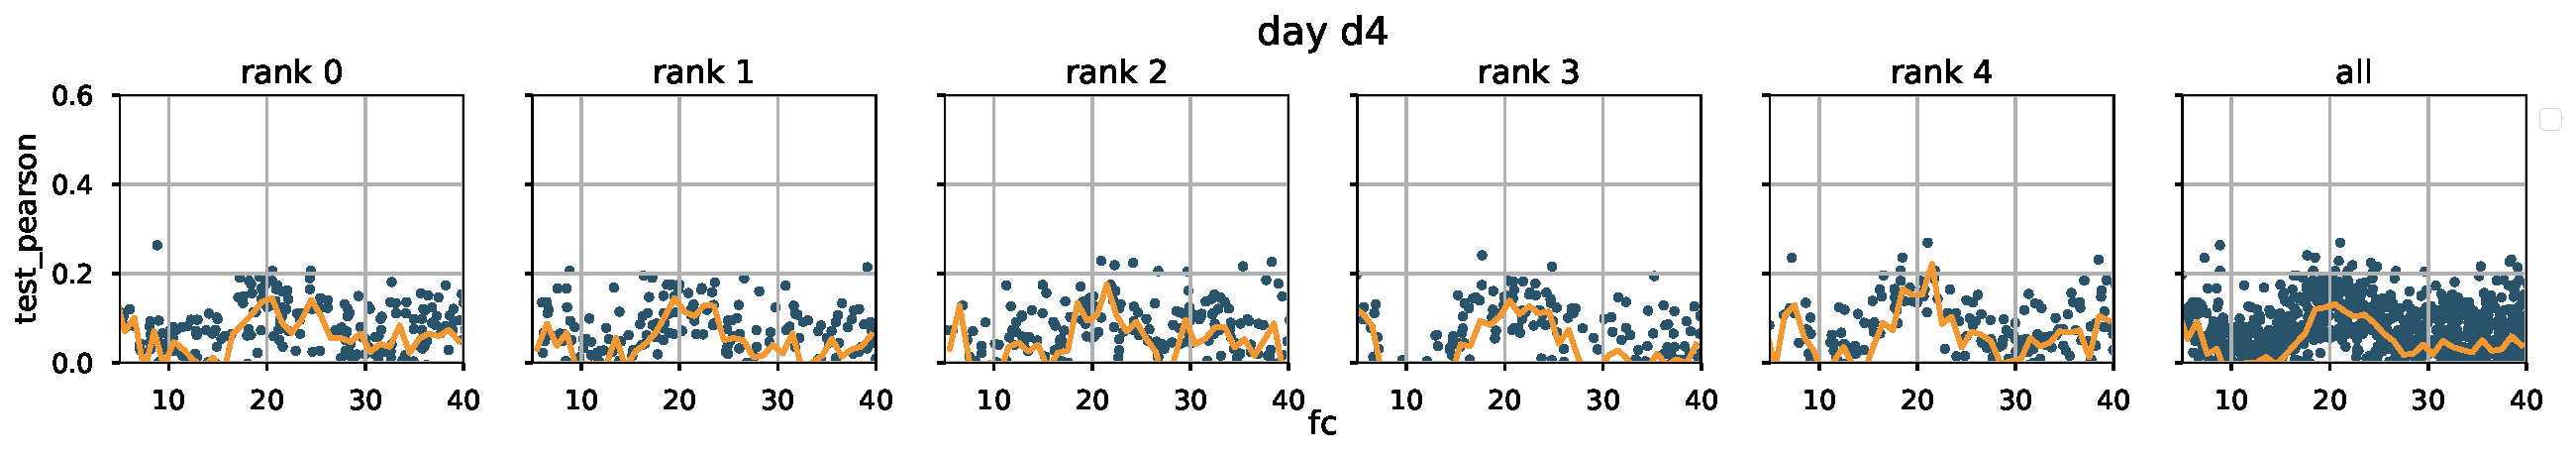
\includegraphics[width=\perfwidth\textwidth]{figures/par_sweep/test_pearson_fc_d4_Shuffle_Single}
\end{tabular}
\caption{Shuffle xval - Pearson - Single} 
\end{figure}
% decoding with spoc (first component) with rho and auc (with ICA)
% using -> all channels / manually selected channels
% rho and auc for components with different ranks

%rho and auc for 1st rank components for different frequency bands

% same plots with SSD

\section{Conclusions}
We have presented a novel framework for the extraction of PD-relevant neural markers

\bibliographystyle{apalike}
\bibliography{specific}

Future work
\begin{itemize}
\item More patients
\item automatic feature extraction (fSPoC?)
\item use LFP data
\end{itemize}

\end{document}